\noindent My empirical analysis integrates farmers' trading records, subjective market expectations, and objective measures of buyer concentration to examine the role of storage in improving smallholder welfare. Specifically, it investigates how storage facilitates inter-temporal arbitrage, allowing farmers to sell in more competitive markets with lower buyer power, an aspect often overlooked in smallholder market research.  

Existing observational data are insufficient, as micro-surveys typically capture post-trade outcomes (e.g., transaction prices, storage volumes) but lack measures of temporal market competitiveness, such as buyer visits and price offer frequency after harvest. A survey-based approach is therefore necessary to assess how farmers' storage decisions and local procurement market structures shape their bargaining power.  

%------------------------------------------------------%
\section{Field Site: A County in Central China}
\noindent This study surveys both farmers and intermediaries in Yanchang County, Shaanxi Province, a region where Fuji apple cultivation dominates (see Figure \ref{Figure: Yanchang}). Given its reliance on a single cash crop and the strategic role of cold storage in marketing decisions, Yanchang provides an ideal setting to analyze the interaction between storage and market competition. Each village has a central market where farmers sell apples to middlemen and traders, with commercial cold storage facilities available for rent. In 2024, the county's fruit storage capacity reached 180,000 tons, with most of it utilized annually.  

\begin{figure}[thp]
\centering
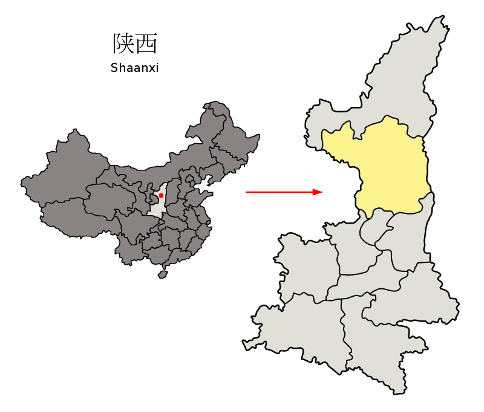
\includegraphics[width=0.6\textwidth]{figures/yanchang_map.png}
\caption{Location of Yanchang County in China}
\label{Figure: Yanchang}
\end{figure}

Yanchang's apple sector is dominated by late-maturing Fuji apples, which account for 85-90\% of total production, alongside smaller shares of mid-maturing (5-10\%) and early-maturing apples (around 5\%) \citep{yanchang2023}. Farm-gate prices range from 2.5 to 12 yuan per kilogram (\$0.16 to \$0.74 per pound) and fluctuate regularly, though yields per acre remain similar across varieties.  

The county consists of over 260 villages across eight rural townships, but cold storage infrastructure is limited. With just over 100 storage facilities, most villages lack direct access. Apple growers primarily use three types of cold storage: self-built facilities (capacity up to 50 tons) and small- and large-sized commercial facilities (up to 500 and 8000 tons, respectively). Only 1.3\% of farmers own storage, relying instead on rentals from township-run or merchant-operated facilities. Government-built storage facilities tend to be of lower quality than farmer-constructed ones. Farmers who build their own storage receive a 40\% government subsidy but must cover the remaining 60\% of the costs.  

Farmers without access to cold storage must sell their harvest within a month, while those with storage can extend sales into April or May, depending on market conditions. Apples stored at 1 degree Celsius in controlled environments maintain quality for several months \citep{Varela2005Shelf-life, Echeverria2004Relationships}. Storage adoption grants farmers temporal flexibility, allowing them to delay sales and potentially access a broader set of buyers, including direct-to-consumer retail markets, rather than being constrained to sell to middlemen. The ability to time sales strategically based on market competition and price fluctuations is a key determinant of storage's economic value.  



%------------------------------------------------------%
%------------------------------------------------------%
\section{Data}
\subsection{Sampling Procedure}
\noindent This study employs empirical tests using data from two rounds of a survey of 615 smallholder apple growers in Yanchang County, Central China, covering the 2024/2025 agricultural season. With Institutional Review Board (IRB) approval, the survey was conducted between October 10, 2024, and December 13, 2024. Since Fuji apple harvest in Central China concludes in mid-to-late October, followed immediately by storage and marketing decisions, this period provides a relevant window to analyze farmers' evolving market conditions.  

The survey was conducted in collaboration with the Yanchang-County Women's Federation (YWF), a local organization focused on public welfare and rural development. In coordination with the Yanchang County Agricultural Bureau, the YWF facilitated access to micro-level data on apple growers, enabling a structured sampling approach. A one-layer stratified random sampling method was applied based on geographical location. To ensure representativeness, the Yanchang County Agricultural Bureau determined sampling proportions for each town (30\%, 15\%, 15\%, 15\%, 10\%, 5\%, 5\%, and 5\%), reflecting the number and density of apple growers. Following these proportions, smallholder apple-growing households were randomly selected from village rosters.\footnote{In Yanchang County, over 95\% of apple growers cultivate no more than five acres, with large-scale commercial orchards being virtually nonexistent. The region is characterized by fragmented landholdings and household-based farming.}  

Smallholder apple growers are defined as those cultivating no more than 50 mu (about 8.24 acres) and deriving at least 90\% of their agricultural income from red Fuji apple production. A minimum of 10 farmers was selected per town to maintain sufficient sample sizes, though no village-level minimum was imposed. Interviews were conducted with household heads unless they were elderly and no longer part of the active labor force, in which case, the primary labor force member was interviewed.  

As indicated in Chapter~\ref{Chapter: descriptive chapter}, the cost of renting cold storage is charged based on weight rather than storage duration. It is therefore a one-time fee incurred at the time of apple storage, typically ranging from 0.4 to 0.6 RMB (5 to 8 cents in US dollars) per kilogram, depending on the type of cold storage facility. Considering that the average harvest price of apples in the region over the past decade has ranged from 4 to 8 RMB (0.55 to 1.10 US dollars) per kilogram, the cold storage rental fee (i.e., the storage cost) accounts for approximately 5\% to 15\% of the harvest price. In other words, if a farmer decides to store, considering other expenses like the transportation cost, he or she needs to get at least 10\% more than the harvest price to make the storage profitable.

%------------------------------------------------------%
\subsection{Measures of Farmers' Storage Usage and Procurement Competitiveness}
\noindent This study examines apple growers' cold storage usage and marketing timing decisions as key dependent variables. First, I define \texttt{Storage-Usage-Binary}, a binary indicator equal to 1 if a farmer used cold storage at harvest and 0 otherwise. Second, \texttt{Storage-Usage-Type} categorizes storage choices into four groups: \textit{Not\_use} (no storage), \textit{Rent\_large} (rented large-scale commercial storage), \textit{Rent\_small} (rented small-scale storage), and \textit{Self\_built} (self-owned storage). Third, \texttt{Time-to-Sell} measures the delay between harvest and sale, effectively capturing storage duration. Sales occurring in October are classified as 1-4 weeks post-harvest, November as 5-8 weeks, and so forth, yielding interval-censored data with four predefined selling-time intervals: 1-4, 5-8, 9-12, and 13-28 weeks. Figure \ref{Figure: selling weeks distribution} illustrates the distribution of selling weeks by storage type.  

\begin{figure}[H]
\centering
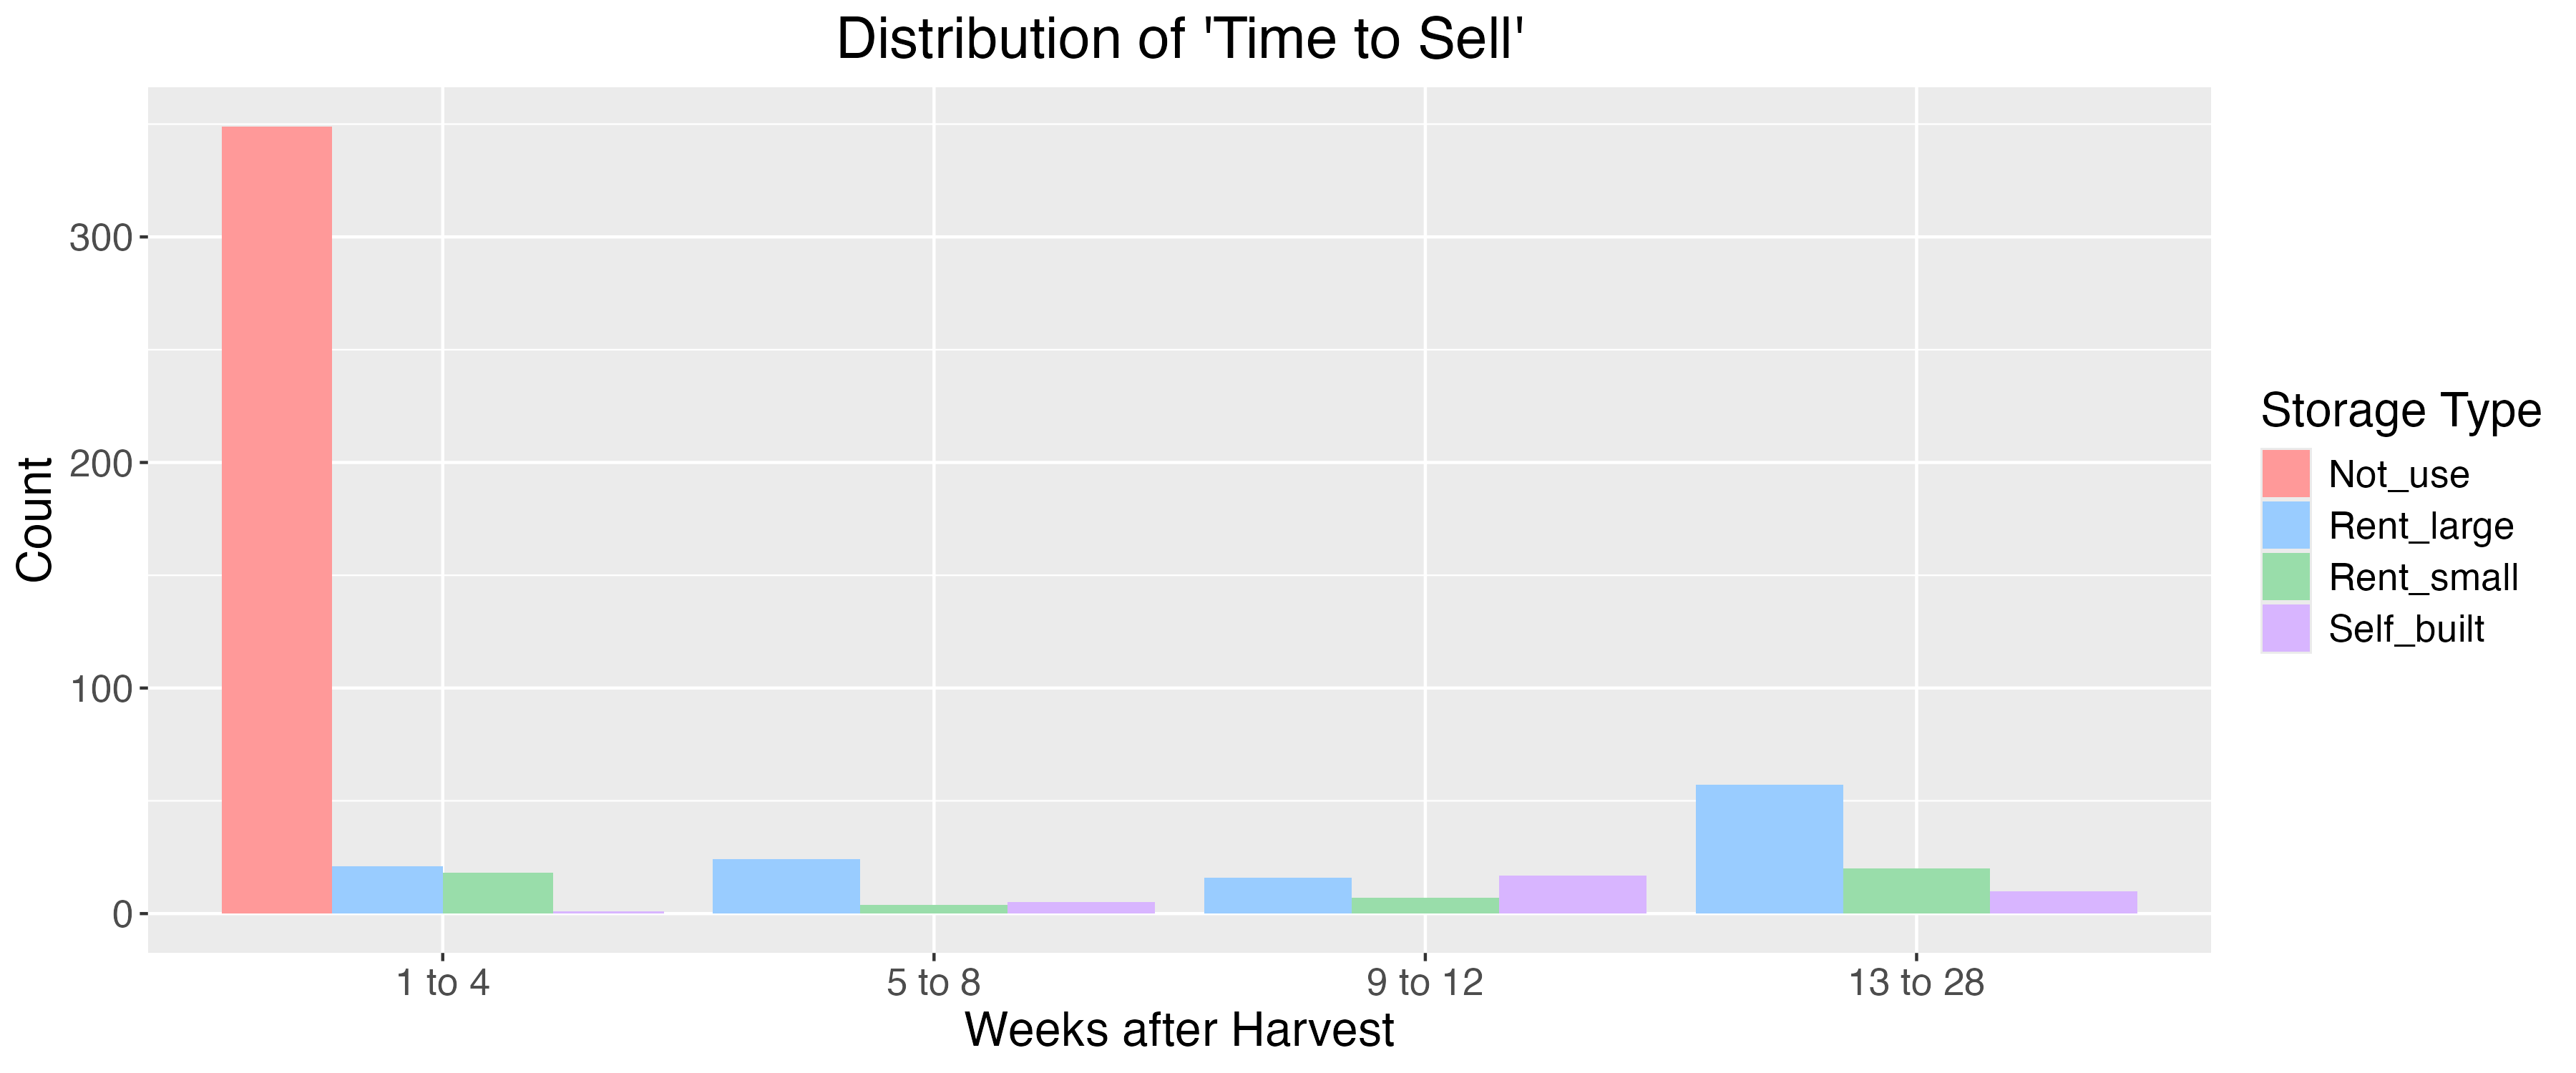
\includegraphics[width=1\textwidth]{figures/selling_weeks_distribution.png}
\caption{Distribution of Selling Weeks by Storage Type}
\label{Figure: selling weeks distribution}
\end{figure}

To capture inter-temporal variations in buyer power and market competitive conditions, farmers reported:
\begin{enumerate}
    \item Their subjective assessment of buyer competition at harvest (\texttt{Subjective buyer competitiveness}, measured on a 1-5 scale);
    \item Their expectations regarding changes in the number of traders over the next three months (recorded as \texttt{Expect more buyers} and \texttt{Expect fewer buyers}).
\end{enumerate}

Additionally, the survey collected data on farmers' agricultural income, production costs, storage expenses, and demographic characteristics to assess the welfare implications of storage adoption.  

To complement these farmer-level insights with market-level dynamics, a buyer survey was conducted in December 2024. This survey targeted 15 buyers, including the top five most influential local traders, and collected data on:
\begin{enumerate}
    \item The specific villages each buyer visited during the October harvest;
    \item The cold storage facilities from which they had procured apples over the preceding two months.
\end{enumerate}
These responses allow for the construction of an objective measure of buyer concentration which might serve as a proxy of inter-temporal buyer competition. Inspired by \cite{macchiavello2021competition}, who used the number of coffee mills within a 10 km radius as a competition metric in Rwanda's coffee industry, I define \texttt{Number of buyers} as the count of traders visiting each village at harvest.  


%------------------------------------------------------%
\subsection{Measures of Farmers' Risk Aversion and Liquidity Constraint}
\noindent Building on \cite{jin2024losses}, whose fieldwork location closely aligns with that of this study, apple growers' risk preferences are measured using two complementary methods: a self-reported risk preference scale and a behavioral measure based on a Holt-Laury-type lottery game. The combination of subjective and incentivized approaches provides a robust assessment of farmers' risk attitudes. Liquidity constraints are defined following \cite{albuquerque2024market} and \cite{stephens2011incomplete}, classifying farmers as liquidity-constrained if they report both difficulty accessing credit and a need to sell immediately at harvest to meet urgent cash requirements.

\subsubsection{Self-Reported Risk Preference}  
\noindent Following \cite{dohmen2011individual}, general risk attitudes are elicited through a five-point scale, where 1 indicates \textit{``extreme risk aversion''} and 5 represents \textit{``very risk loving''}. While inherently subjective and potentially influenced by social and peer effects, self-reported measures provide useful insights into farmers' perceptions of risk, which likely influence investment, production, and financial decisions.  

\subsubsection{Holt-Laury-Type Lottery Game}  
\noindent To complement the self-assessment, a modified Holt-Laury-type lottery game was implemented. Apple growers were asked how much they would be willing to pay to enter a 50-50 lottery with a potential payout of 200 CNY or nothing. This adapts the \textit{multiple price list (MPL) choice task} from \cite{brick2012risk}, a variation of the Holt-Laury method \citep{holt2002risk}. Participants chose whether to pay varying entry fees (20-120 CNY), effectively selecting between a \textit{safe} (keeping the money) and a \textit{risky} (entering the lottery) option.  

This approach is well-suited for field settings, being simple to administer while using real monetary stakes to elicit truthful responses. Different willingness-to-pay (WTP) values correspond to varying expected values and degrees of risk aversion, as shown in Table \ref{tab:experiment_design}.  

\begin{table}[H]
    \centering
    \footnotesize 
    \caption{Risk Preference Experiment Design: A Head-Tail Lottery Game}
    \renewcommand{\arraystretch}{1.2}
    \begin{tabular}{cccccc}
        \toprule
        \textbf{Option} & \textbf{Willingness to Pay} & \textbf{Outcome} & \textbf{EV$^{A}$--EV$^{B}$} & \textbf{CRRA Ranges} & \textbf{CRRA Adjusted}\\
        \midrule
        1 & 120 CNY & 200 CNY or 0 & 20 CNY & $-0.4 < \gamma < 0$  & $\gamma = -0.2$\\
        2 & 100 CNY & 200 CNY or 0 & 0 CNY & $0 < \gamma < 0.2$  & $\gamma= 0.1$ \\
        3 & 80 CNY & 200 CNY or 0 & -20 CNY & $0.2 < \gamma < 0.4$  & $\gamma= 0.3$ \\
        4 & 60 CNY & 200 CNY or 0 & -40 CNY & $0.4 < \gamma < 0.6$  & $\gamma= 0.5$ \\
        5 & 40 CNY & 200 CNY or 0 & -60 CNY & $0.6 < \gamma < 0.7$  & $\gamma=0.6$ \\
        6 & 20 CNY & 200 CNY or 0 & -80 CNY & $0.7 < \gamma$  & $\gamma= 0.9$ \\
        \bottomrule
    \end{tabular}
    \label{tab:experiment_design}
    \vspace{0.5em}
    \small Notes: EV = Expected Value. CRRA = Coefficient of Constant Relative Risk Aversion.
\end{table}

While the head-tail lottery design provides a tractable way to elicit \textit{point estimates} of risk preferences in the field, the implied CRRA coefficients are typically much smaller than the range used in simulation exercises. For instance, the experimental design in Table~\ref{tab:experiment_design} maps observed willingness-to-pay decisions into CRRA values that mostly fall below 1, consistent with evidence from other MPL-style tasks in agricultural settings. By contrast, the simulations in Section~\ref{Section: Base Model Numerical Analysis} in Chapter 4 vary $\gamma$ over a wider domain, $[0,10]$, to capture the full spectrum of heterogeneity documented in the literature---from risk neutrality to extreme risk aversion. In practice, the field experiment serves to benchmark farmers' risk preferences around the lower end of this spectrum, while the simulation framework explores the implications of more severe risk aversion that, although less common, is empirically observed in some rural populations.\footnote{Empirical studies using similar elicitation tasks often report CRRA values in the range of 0.5--3 (see, e.g., \cite{liu2013time}).}



\subsubsection{Estimating Risk Aversion Using CRRA}  
\noindent The highest entry price a participant is willing to pay provides insight into their risk preference. Following \cite{chiappori2011relative}, who found that individuals generally exhibit constant relative risk aversion (CRRA), a CRRA utility function is assumed:  
\[
U(x) = \frac{x^{1-\gamma}}{1 - \gamma}
\]  
where \( \gamma \) represents the risk aversion coefficient. Under this specification, \( \gamma > 0 \) implies risk aversion, \( \gamma = 0 \) indicates risk neutrality, and \( \gamma < 0 \) reflects risk-seeking behavior. Columns 5 and 6 in Table \ref{tab:experiment_design} present the corresponding CRRA ranges and adjusted CRRA values. These estimates allow for a quantitative assessment of farmers' risk aversion, which is critical for understanding storage decisions and responses to market uncertainty.  

\subsubsection{Liquidity Constraint}  
\noindent The binary variable \texttt{Liquidity constrained} equals 1 if a farmer reports both difficulty accessing credit and an urgent need to sell at harvest to cover immediate expenses (e.g., school tuition or medical costs). This measure refines and extends approaches used by \cite{albuquerque2024market} and \cite{stephens2011incomplete}, who define credit access as a proxy for liquidity constraints.  

Only a small fraction of surveyed farmers (about 15\%) meet the criteria for liquidity constraints, with no strong correlation between liquidity constraints and storage or selling decisions. One possible explanation is that the study region, located in Central China, is a designated provincial rural revitalization area, attracting both state- and private-owned financial institutions that provide inclusive credit access.  

Additionally, insights from interviewed local villagers suggest that past exposure to natural disasters, such as hailstorms, has fostered a strong savings culture. Farmers in Yanchang County prioritize financial resilience, making them less likely to engage in distress sales. While liquidity constraints affect some growers, this measure primarily captures relative financial strain rather than absolute financial distress.  




%------------------------------------------------------%
\subsection{Descriptive Statistics}  
\noindent The final dataset consists of 549 smallholder apple-growing households in Central China, of whom 200 used cold storage during the 2024-2025 agricultural year. Among these, 33 stored apples in self-built facilities, 49 rented small-scale commercial storage, and 118 opted for large-scale commercial storage.  

\begin{figure}[htp]
\centering
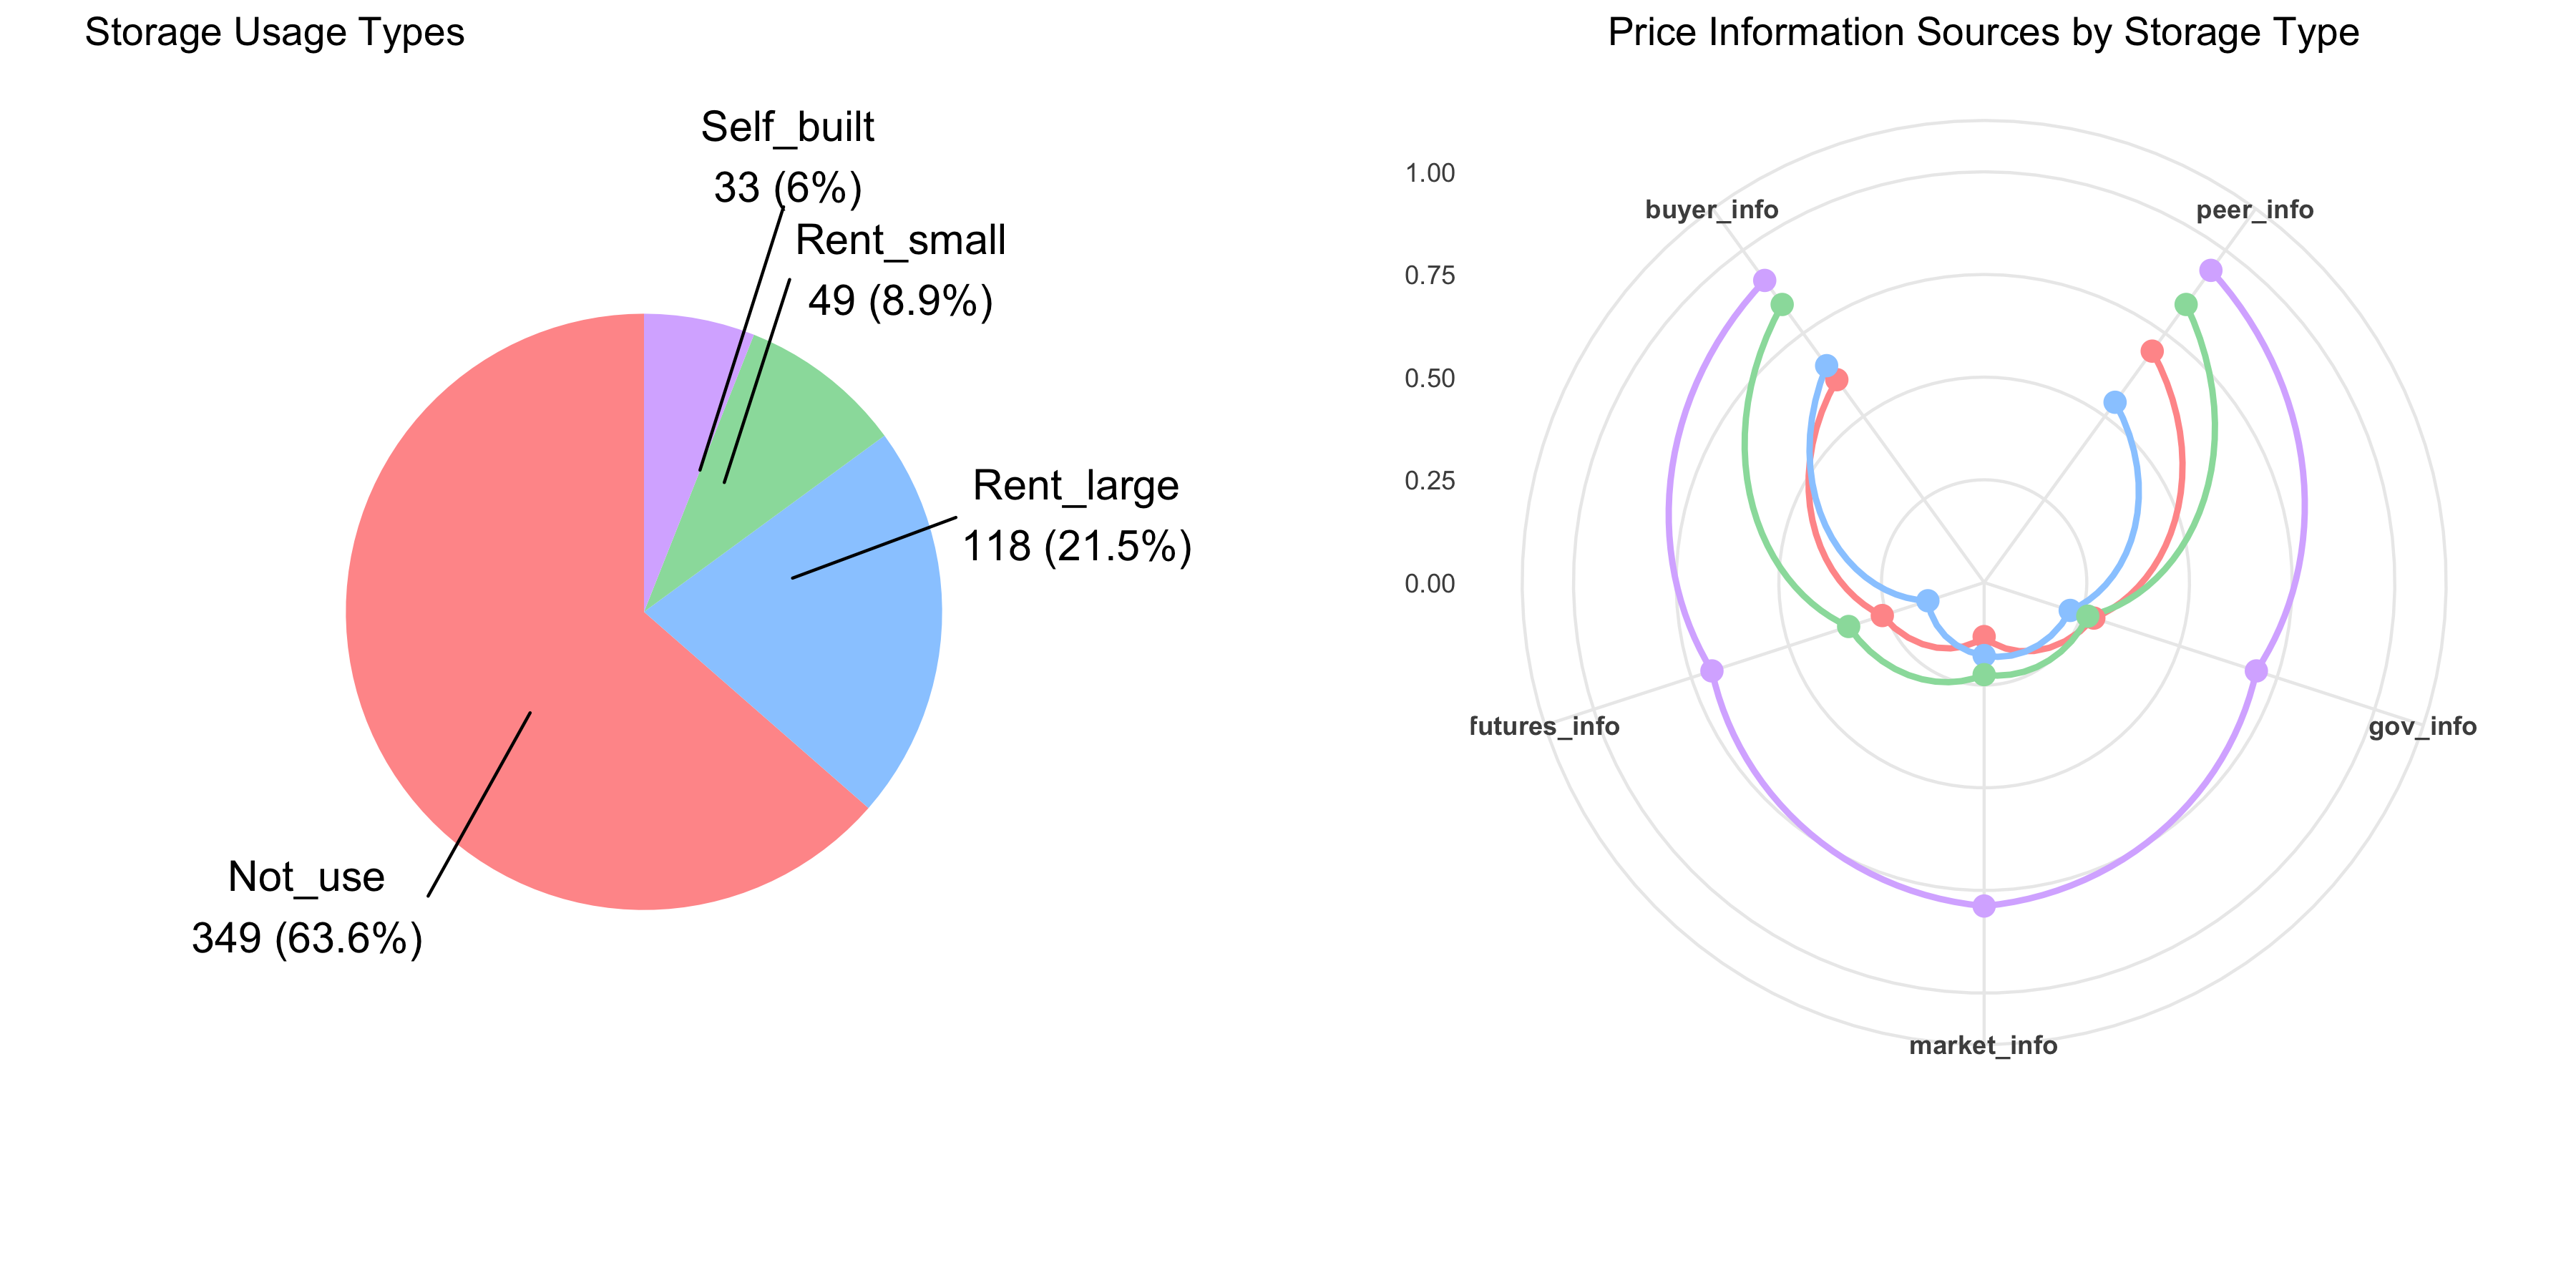
\includegraphics[width=1\textwidth]{figures/storage_usage_analysis_soft_colors.png}
\caption{Distribution of Storage Usage Types and Their Price Information Sources}
\label{Figure: pie and radar chart}
\end{figure}

Figure \ref{Figure: pie and radar chart} illustrates the distribution of storage usage and the sources of price information. The radar chart on the right highlights variations in information-seeking behavior across groups. Growers with self-built storage (purple) are the most active in gathering market insights, suggesting a strong need for independent decision-making. Those using small-scale (green) and large-scale (blue) commercial storage engage at moderate but balanced levels, likely reflecting a reliance on both direct transactions and broader market signals. In contrast, growers selling immediately at harvest (red) show minimal engagement, primarily depending on buyer and peer information.  

These differences in search activity are also reflected in the composition of price information sources. Self-built storage users prioritize market data while supplementing it with buyer and peer sources, aligning with their need to optimize sales timing. Small-scale commercial users rely heavily on buyer and peer information, reflecting localized transactions and network-based decision-making. Large-scale commercial users adopt a more diversified approach, integrating multiple sources to manage risk and maximize returns. Growers selling at harvest depend narrowly on immediate contacts for pricing, underusing institutional sources such as government data and futures markets. This pattern suggests a general preference for informal, experience-based price discovery over structured, institutional sources.

\begin{table}[H]
\centering
\caption{Summary Statistics by Storage Usage}
\label{tab: summary statistics}
\resizebox{\textwidth}{!}{%
\begin{tabular}{lccccc}
\toprule
 & \multicolumn{2}{c}{Storage Users} & \multicolumn{2}{c}{Non-Users} & Difference \\
\cmidrule(lr){2-3} \cmidrule(lr){4-5}
Variable & Mean & SD & Mean & SD & t-statistic \\
\midrule
\multicolumn{6}{l}{\textbf{Panel A: Farmer Demographics}} \\
Age (years) & 56.87 & (9.57) & 60.35 & (9.63) & -4.09*** \\
Household size (persons) & 2.71 & (1.21) & 2.58 & (1.10) & 1.24 \\
Labor size (persons) & 1.74 & (0.71) & 1.60 & (0.66) & 2.20** \\
Highest education (level) & 1.96 & (0.67) & 1.81 & (0.76) & 2.35** \\
Family ever village leader (0/1) & 0.24 & (0.43) & 0.06 & (0.24) & 5.37*** \\
Liquidity constrained (0/1) & 0.15 & (0.36) & 0.16 & (0.37) & -0.17 \\
\addlinespace
\multicolumn{6}{l}{\textbf{Panel B: Production and Consumption}} \\
Apple yield (tons) & 11.08 & (7.56) & 11.68 & (14.12) & -0.64 \\
Land size (acre) & 2.60 & (1.70) & 1.72 & (0.99) & 6.69*** \\
Bad apple ratio & 2.31 & (1.20) & 2.02 & (1.18) & 2.78*** \\
Apple income (USD) & 10127.22 & (6108) & 8289 & (6465) & 3.32*** \\
Total income (USD) & 10919 & (6445) & 8990 & (7334) & 3.21*** \\
Labor cost (USD) & 1911 & (1593) & 1343 & (1258) & 4.33*** \\
Family consumption (USD) & 7117 & (8899) & 5059 & (3869) & 3.11*** \\
\addlinespace
\multicolumn{6}{l}{\textbf{Panel C: Storage and Risk-Related Factors}} \\
Car/truck ownership (0/1) & 0.14 & (0.35) & 0.04 & (0.20) & 3.61*** \\
Natural disaster insurance (0/1) & 0.35 & (0.48) & 0.33 & (0.47) & 0.49 \\
Price insurance (0/1) & 0.62 & (0.49) & 0.65 & (0.48) & -0.78 \\
CRRA adjusted (coef) & 0.09 & (0.37) & 0.36 & (0.45) & -7.75*** \\
Storage in village (0/1) & 0.38 & (0.49) & 0.20 & (0.60) & 3.74*** \\
Far to small storage (0/1) & 0.52 & (0.50) & 0.79 & (0.41) & -6.71*** \\
Far to large storage (0/1) & 0.89 & (0.32) & 0.91 & (0.28) & -1.07 \\
Storage for wider marketing (0/1) & 0.88 & (0.33) & 0.30 & (0.46) & 16.90*** \\
Storage as bargaining tool (0/1) & 0.80 & (0.40) & 0.29 & (0.46) & 13.79*** \\
\addlinespace
\multicolumn{6}{l}{\textbf{Panel D: Marketing}} \\
Highest price per pound (USD/lb) & 0.41 & (0.09) & 0.38 & (0.10) & 3.94*** \\
Good price per pound (USD/lb) & 0.40 & (0.08) & 0.37 & (0.10) & 3.29*** \\
WeChat selling (0/1) & 0.15 & (0.36) & 0.00 & (0.00) & 6.04*** \\
Relational selling (0/1) & 0.12 & (0.33) & 0.14 & (0.35) & -0.78 \\
Contract selling (0/1) & 0.40 & (0.49) & 0.26 & (0.44) & 3.32*** \\
\addlinespace
\multicolumn{6}{l}{\textbf{Panel E: Market Competitive Conditions}} \\
Expect more buyers (0/1) & 0.46 & (0.50) & 0.06 & (0.23) & 10.75*** \\
Expect fewer buyers (0/1) & 0.16 & (0.39) & 0.19 & (0.39) & -0.90 \\
Number of buyers at harvest (count) & 3.83 & (2.45) & 3.12 & (1.91) & 3.51*** \\
Subjective buyer competitiveness (1/5) & 2.92 & (0.84) & 3.06 & (0.69) & -2.08** \\
\hline
\hline
Observations & 200 & & 349 & & 549 \\
\bottomrule
\end{tabular}% 
} % End of resizebox 
\begin{tablenotes} 
\item \textit{Notes:} The table presents means and standard deviations (in parentheses) for each variable by group. T-statistics from two-sample t-tests are reported to indicate statistical significance of differences between groups. Significance levels are denoted by asterisks: * p$<$0.1, ** p$<$0.05, *** p$<$0.01. In addition, monetary values have been converted from Chinese Yuan (RMB) to US Dollars (USD), land area from mu to acres, and apple prices from RMB/kg to USD/pound using appropriate conversion rates. 
\end{tablenotes} 
\end{table}


The subset of 200 storage users provides a key sample for analyzing storage-related decision-making in greater detail. Table \ref{tab: summary statistics} presents descriptive statistics comparing storage users and non-users across key demographic, production, marketing, and market competition variables. Significant differences emerge in demographic characteristics, with storage users being younger on average (56.87 vs. 60.35 years, $p < 0.01$), having slightly larger household labor forces (1.74 vs. 1.60 persons, $p < 0.05$), and being more likely to have a family member who has served as a village leader (24\% vs. 6\%, $p < 0.01$). While education levels are marginally higher for storage users (1.96 vs. 1.81 on a categorical scale, $p < 0.05$), liquidity constraints appear similar across both groups. These findings suggest that access to storage may be associated with leadership connections and greater household labor availability, which could facilitate better market participation and bargaining power. The rightmost column reports t-statistics from two-sample t-tests to indicate whether differences between groups are statistically significant.  

In terms of production and income, storage users operate on significantly larger landholdings (2.60 vs. 1.72 acres, $p < 0.01$) and report higher apple-related earnings (\$10,127 vs. \$8,289, $p < 0.01$). However, their yields per acre do not significantly differ from non-users. Storage users also face a slightly higher proportion of bad apples (2.31 vs. 2.02, $p < 0.01$), suggesting that storage may play a role in mitigating losses from quality deterioration. Additionally, storage users incur greater labor costs (\$1,911 vs. \$1,343, $p < 0.01$) and spend more on family consumption (\$7,117 vs. \$5,059, $p < 0.01$).  

Storage access appears closely linked to marketing strategy and market expectations. A significantly larger proportion of storage users engage in relational selling (40\% vs. 26\%, $p < 0.01$), use WeChat for sales (15\% vs. 0\%, $p < 0.01$), and expect more buyers in the future (46\% vs. 6\%, $p < 0.01$), reflecting greater confidence in market expansion. Moreover, storage enables broader marketing strategies, with 88\% of storage users explicitly storing apples for wider marketing (vs. 30\% among non-users, $p < 0.01$) and 80\% using storage as a bargaining tool (vs. 29\%, $p < 0.01$). These differences suggest that storage is not only a means of extending the sales period but also a strategic tool for improving price negotiation and expanding market reach, reinforcing its role in enhancing producer bargaining power.  

\begin{figure}[htp]
\centering
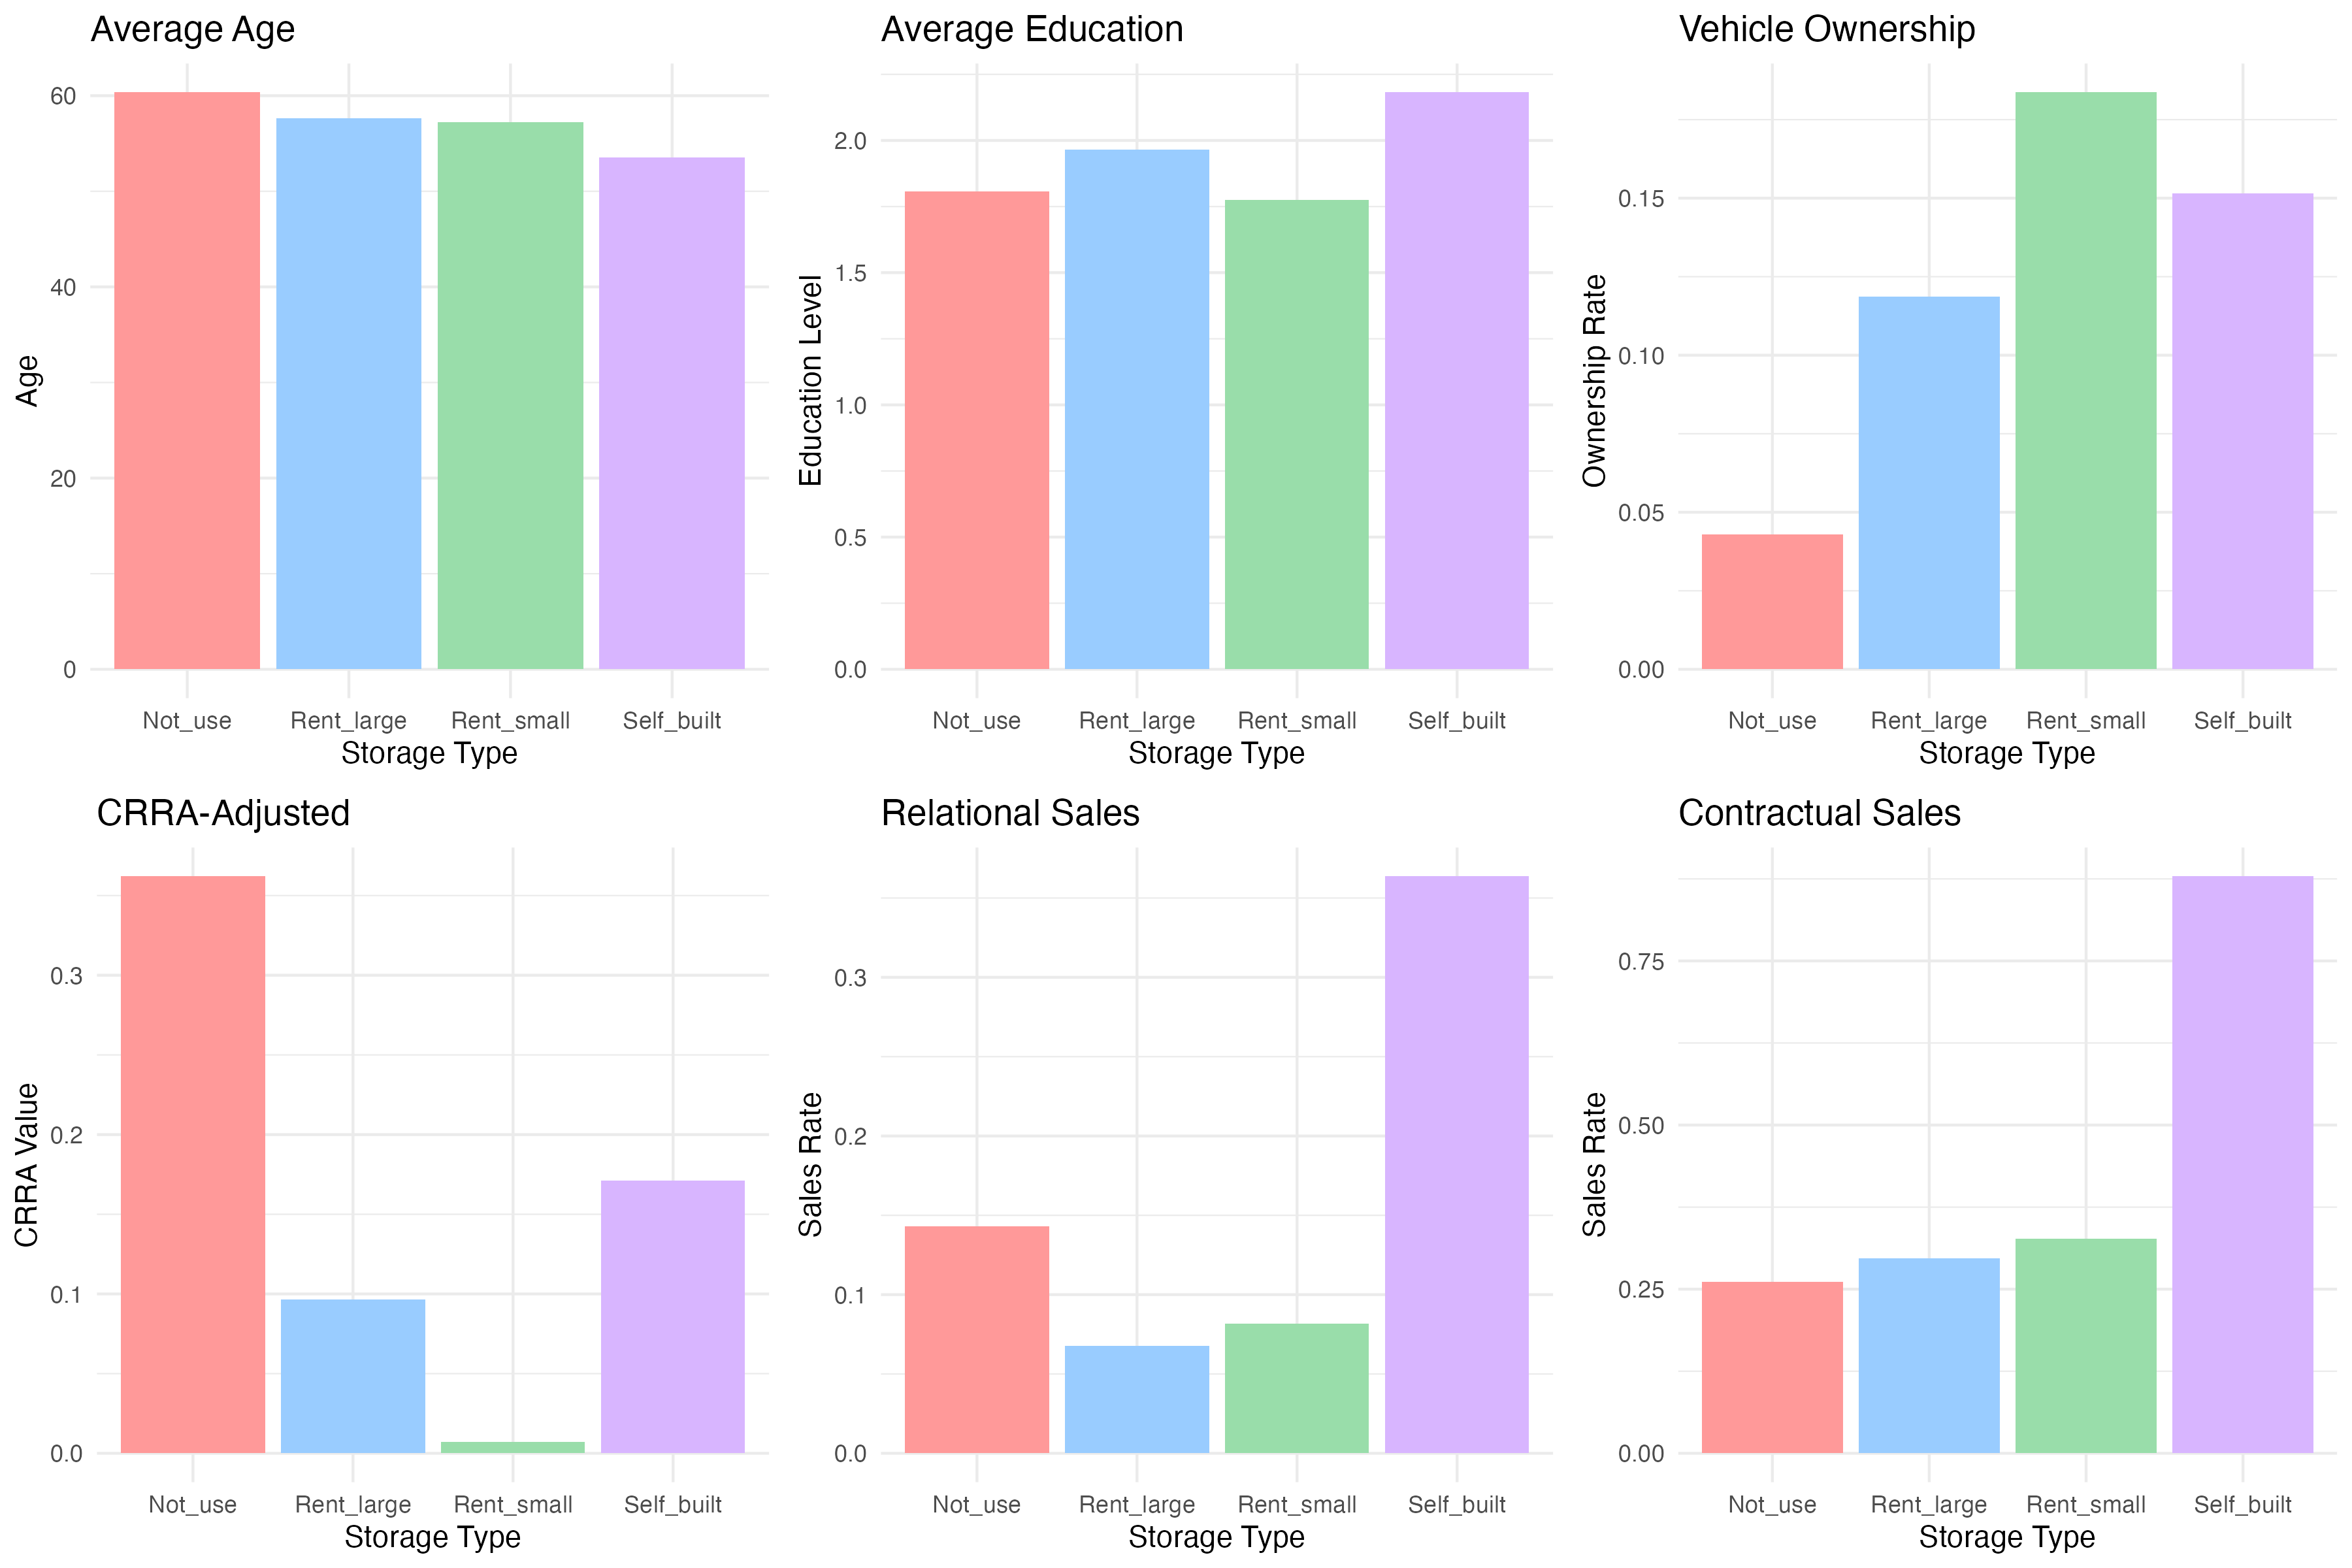
\includegraphics[width=1\textwidth]{figures/combined_storage_metrics.png}
\caption{Demographics by Storage Type}
\label{Figure: Demographics by Storage Type}
\end{figure}

Furthermore, Figure \ref{Figure: Demographics by Storage Type} compares key demographic characteristics across four storage usage categories: non-users, users with self-built storage, and users renting small- and large-scale commercial storage facilities. The figure highlights differences in six key variables: age, education level, car/truck ownership, risk aversion (adjusted CRRA), and participation in relational and implicit contractual sales.   

Table \ref{tab: summary statistics} shows that non-storage farmers receive an average highest price of \$0.38 per pound (6.12 RMB/kg), with an average transaction price of \$0.37 per pound (5.96 RMB/kg), both slightly lower than those of storage users. As illustrated in Figure \ref{Figure: selling price bubble}, non-storage farmers are constrained to selling at harvest (October), when transaction prices exhibit high volatility before stabilizing in subsequent months. Prices typically rise in November and December, though sales volumes decline. Storage users who delay sales achieve on average a price premium of roughly \$0.03 per pound ($\approx$ 0.45 RMB/kg) over non-storers. Given that reported storage costs fall in the same range (0.40-0.50 RMB/kg), the average net payoff to storage in this survey year was close to zero. Nevertheless, storers retained the opportunity to capture substantially higher returns in certain months, with realized prices occasionally reaching \$0.50--\$0.60 per pound ($\approx$ 7.80--9.4 RMB/kg) in December. This highlights the role of storage as a risky inter-temporal strategy: while not systematically profitable on average once costs are deducted, it provided upside potential for some farmers depending on timing and market conditions.


\begin{figure}[H]
\centering
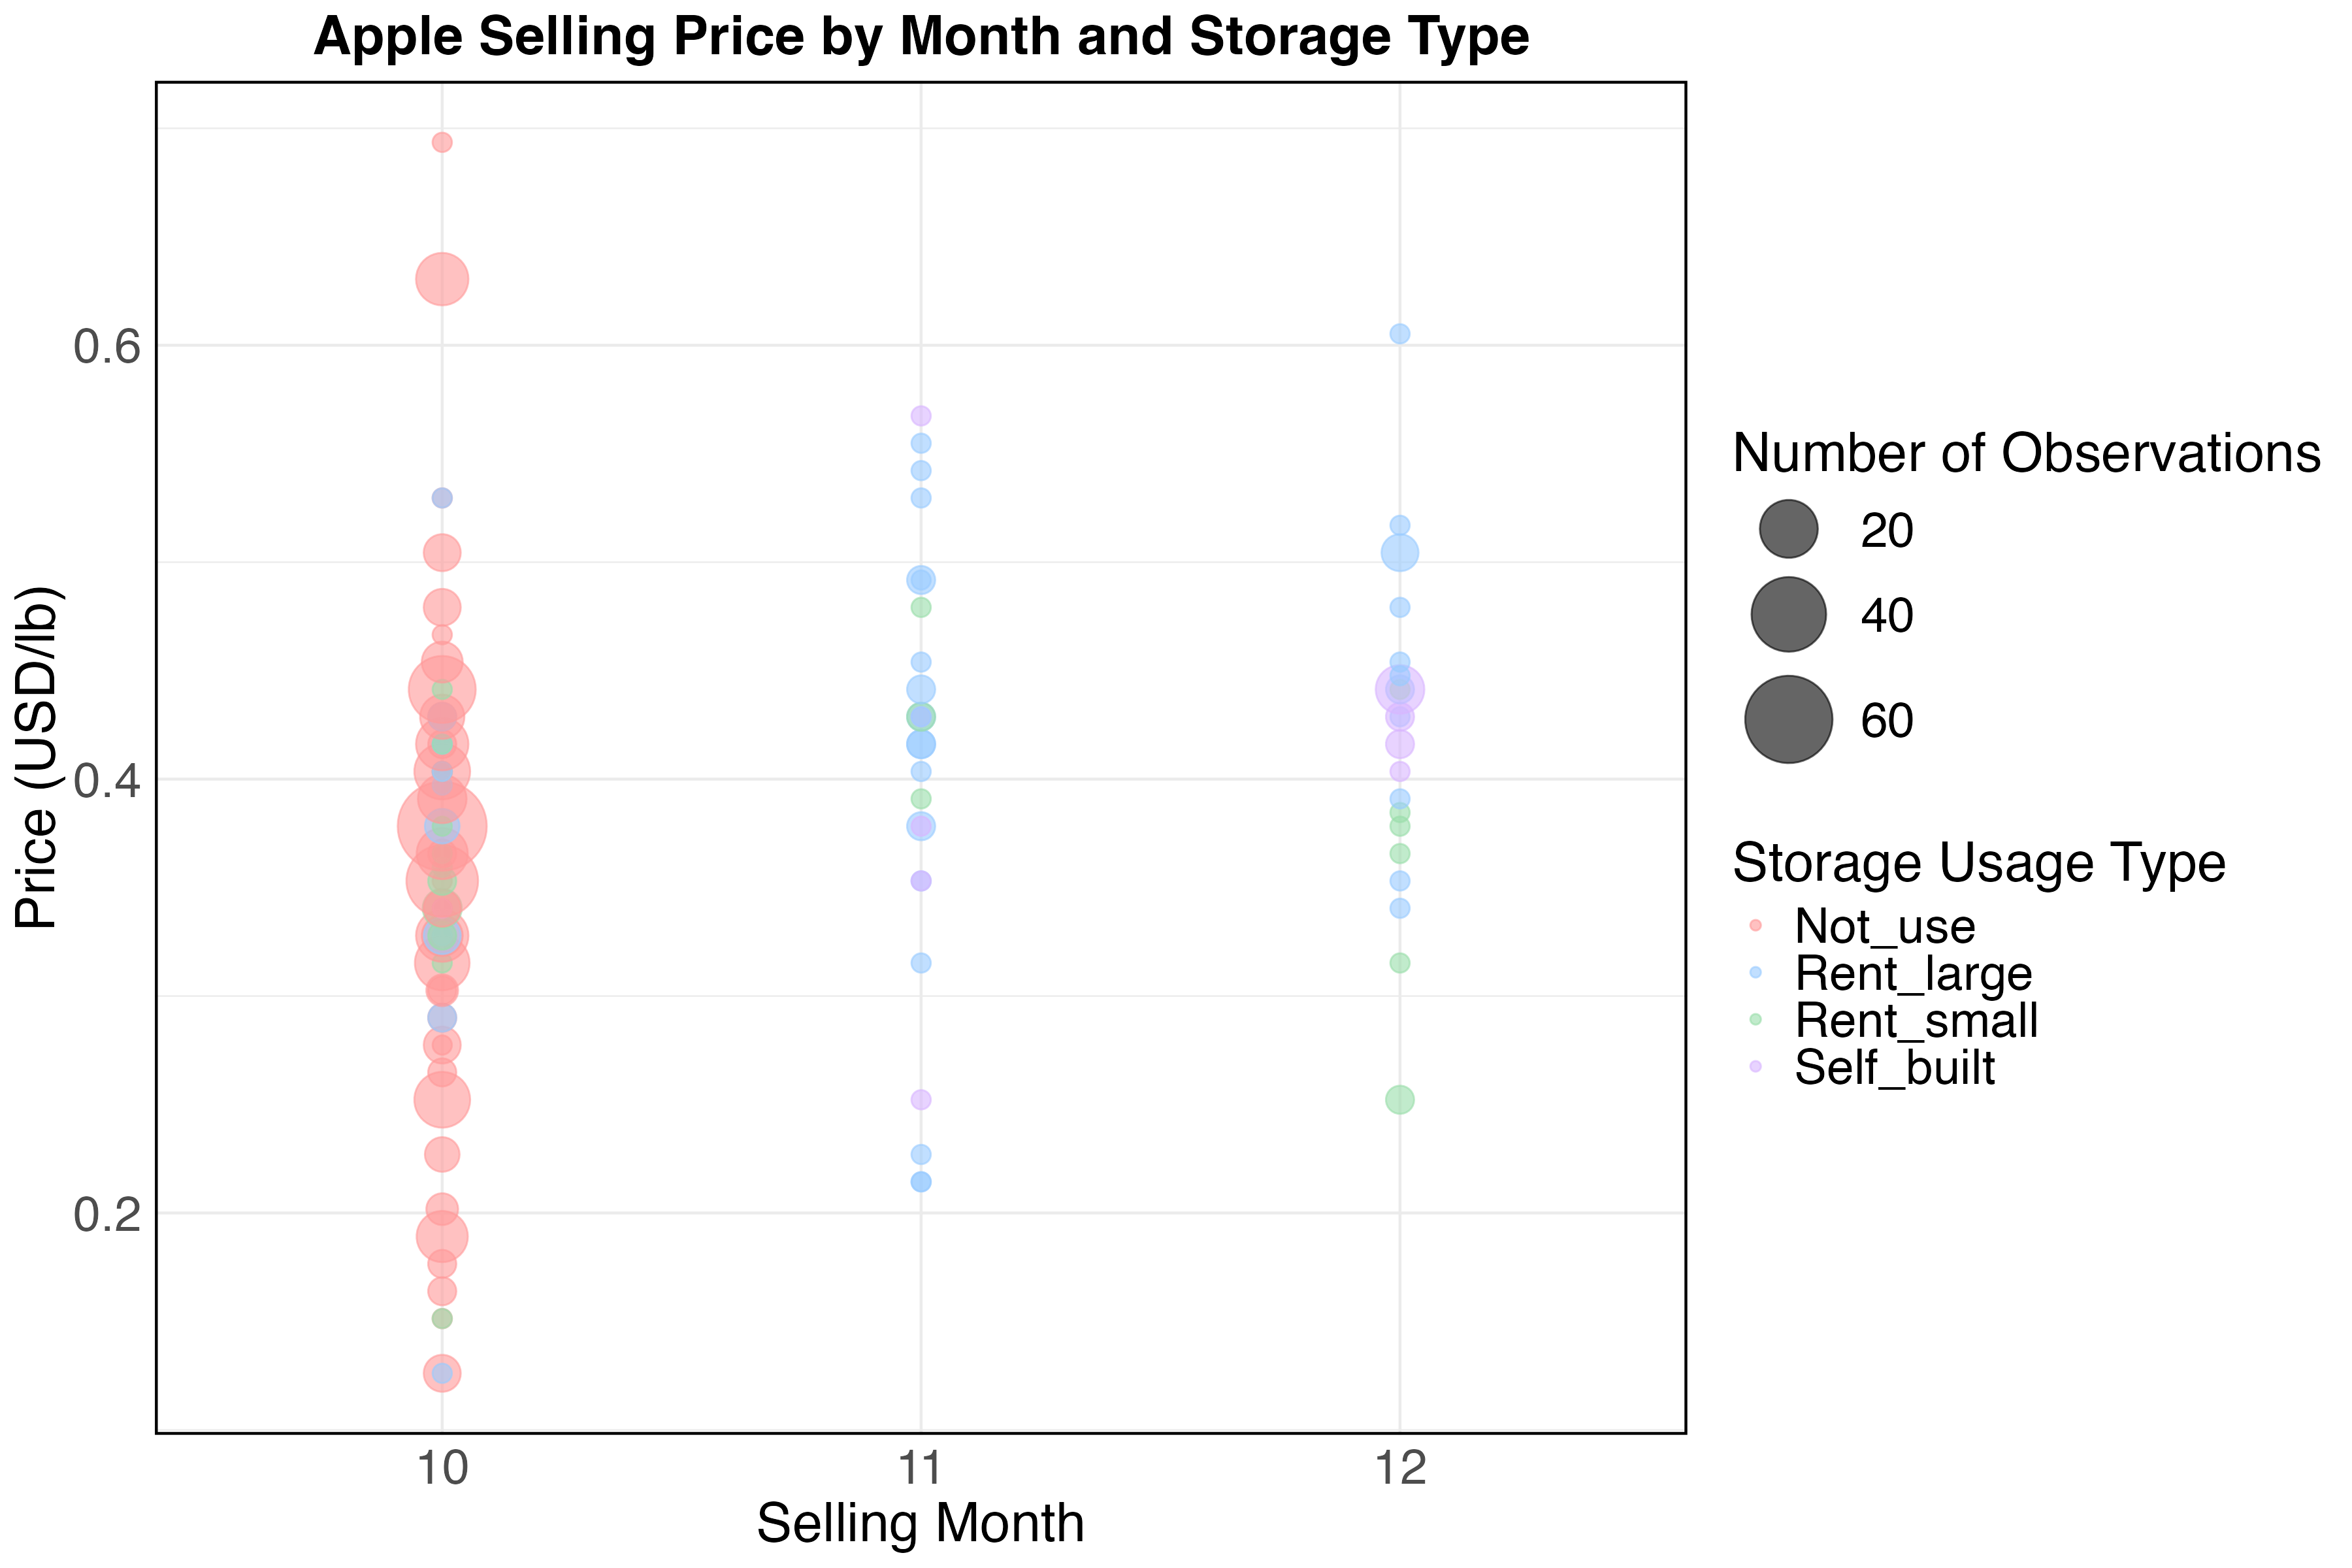
\includegraphics[width=1.05\textwidth]{figures/apple_price_bubble_plot.png}
\caption{Apple Selling Price by Month and Storage Type}
\label{Figure: selling price bubble}
\end{figure}

Despite the potential benefits of storage, many farmers opt not to store their produce, often due to negative past experiences. Table \ref{tab:non_storage_reasons} summarizes the primary reasons cited by 349 non-storage farmers. The most frequently mentioned concern, reported by 60.75\% of respondents, is skepticism about future price increases. Beyond price uncertainty, 28.65\% of farmers perceive storage as too risky, citing potential losses from spoilage, market downturns, or unreliable storage access. Additionally, 22.92\% report high storage costs as a prohibitive factor. A smaller group (8.02\%) indicates that pre-arranged sales eliminate the need for storage. These findings suggest that, while cold storage could improve farmers' marketing flexibility, adoption is hindered by market uncertainty, perceived financial and logistical concerns, and established pre-arranged sales.  


\begin{table}[H]
    \centering
    \footnotesize
    \caption{Reasons for Not Using Storage Facilities}
    \label{tab:non_storage_reasons}
    \resizebox{\textwidth}{!}{%
        \begin{tabular}{lcccc}
            \toprule
            \textbf{Reason} & High Storage Costs & Pre-arranged sale & Cannot Sell High Later & Too Risky \\
            \midrule
            \textbf{Percentage} & 22.92\% & 8.02\% & 60.75\% & 28.65\% \\
            \bottomrule
        \end{tabular}%
        }
        \begin{tablenotes}
            \item \textit{Notes:} This table presents the reasons provided by the 349 farmers who do not use storage facilities, expressed as percentages of total non-storage farmers.
        \end{tablenotes}
\end{table}


%------------------------------------------------------%
%------------------------------------------------------%
\section{Empirical Specification}
\subsection{Storage Decisions: Buyers' Competitiveness at Harvest}
\noindent 
This section presents the results of a logistic regression model with town-level fixed effects examining the determinants of binary storage usage. The dependent variable is whether an individual engages in storage ($S_i = 1$) or not ($S_i = 0$). The key independent variables fall into two categories:  
\begin{enumerate}
    \item \textbf{Subjective beliefs about buyer competition at harvest} ($B^s_i$), measured on a scale from 1 to 5, where higher values indicate stronger perceived competition.  
    \item \textbf{The objective number of buyers at harvest} ($B^o_i$), representing the actual market structure farmers face. 
\end{enumerate}
The estimated logit model with town-level fixed effects is specified as follows:

\begin{equation}
\text{logit} \left( D(S_i= 1) \right) = \beta_0 + \beta_1 B^o_i + \beta_2 B^s_i + \beta_3 X_i + \gamma_\tau + \varepsilon_i
\label{Eq: empirical first one}
\end{equation}
where $D(S_i=1)$ is the dummy variable of storage usage, $X_i$ represents a vector of control variables including demographic and risk-related factors, $\gamma_\tau$ denotes town-level fixed effects, and $\varepsilon_i$ is the error term.  


For completeness, the full set of estimated logit coefficients including control variables is reported in Table \ref{tab: binary storage ~ buyers' competition at harvest}, while Table \ref{tab:marginal_effects_model3} presents the corresponding average marginal effects for ease of interpretation.  

Among the three logistic regression models reported in Table~\ref{tab: binary storage ~ buyers' competition at harvest}, Model 3 is selected as the preferred specification as strikes the best balance: it substantially improves model fit relative to Models 1 and 2 (with an AIC of 460.20 and BIC of 498.97) while maintaining a more parsimonious structure focused on the main effects. Both the number of buyers and subjective beliefs are statistically significant and align with theoretical expectations.


% Table created by stargazer v.5.2.3 by Marek Hlavac, Social Policy Institute. E-mail: marek.hlavac at gmail.com
% Date and time: Wed, Sep 24, 2025 - 19:45:19
\begin{table}[H] \centering 
  \caption{Logistic Regression Results} 
  \label{tab: binary storage ~ buyers' competition at harvest} 
\footnotesize 
\begin{tabular}{@{\extracolsep{5pt}}lccc} 
\\[-1.8ex]\hline 
\hline \\[-1.8ex] 
 & \multicolumn{3}{c}{\textit{Dependent variable:}} \\ 
\cline{2-4} 
\\[-1.8ex] & \multicolumn{3}{c}{Storage Usage (Binary)} \\ 
 & Model 1 & Model 2 & Model 3 \\ 
\\[-1.8ex] & (1) & (2) & (3)\\ 
\hline \\[-1.8ex] 
 Number of Buyers & 0.004 &  & 0.45$^{***}$ \\ 
  & (0.05) &  & (0.10) \\ 
  & & & \\ 
 Subjective Belief &  & $-$0.52$^{***}$ & $-$1.55$^{***}$ \\ 
  &  & (0.16) & (0.28) \\ 
  & & & \\ 
 Age & $-$0.03$^{**}$ & $-$0.03$^{**}$ & $-$0.02$^{*}$ \\ 
  & (0.01) & (0.01) & (0.01) \\ 
  & & & \\ 
 Education Level & 0.38$^{**}$ & 0.36$^{**}$ & 0.31$^{*}$ \\ 
  & (0.17) & (0.17) & (0.18) \\ 
  & & & \\ 
 Family Village Leader & 1.26$^{***}$ & 1.23$^{***}$ & 1.17$^{***}$ \\ 
  & (0.35) & (0.35) & (0.36) \\ 
  & & & \\ 
 CRRA Adjusted & $-$1.08$^{***}$ & $-$0.96$^{***}$ & $-$0.99$^{***}$ \\ 
  & (0.29) & (0.29) & (0.30) \\ 
  & & & \\ 
 Liquidity Constrained & 0.05 & $-$0.05 & $-$0.03 \\ 
  & (0.31) & (0.32) & (0.33) \\ 
  & & & \\ 
 Constant & $-$0.80 & 0.86 & 2.37$^{*}$ \\ 
  & (1.06) & (1.18) & (1.21) \\ 
  & & & \\ 
\hline \\[-1.8ex] 
Town Fixed Effects & Yes & Yes & Yes \\ 
Observations & 549 & 549 & 549 \\ 
Log Likelihood & $-$237.94 & $-$232.29 & $-$221.10 \\ 
Akaike Inf. Crit. & 491.88 & 480.58 & 460.20 \\ 
Bayesian Inf. Crit. & 526.34 & 515.04 & 498.97 \\ 
\hline 
\hline \\[-1.8ex] 
\textit{Note:}  & \multicolumn{3}{r}{$^{*}$p$<$0.1; $^{**}$p$<$0.05; $^{***}$p$<$0.01} \\ 
\end{tabular} 
\end{table} 


\begin{table}[H] \centering 
  \caption{Average Marginal Effects from Logistic Regression (Model 3)} 
  \label{tab:marginal_effects_model3} 
\footnotesize 
\begin{tabular}{@{\extracolsep{5pt}} cc} 
\\[-1.8ex]\hline 
\hline \\[-1.8ex] 
Variable & AME (SE) \\ 
\hline \\[-1.8ex] 
Number of Buyers at harvest & 0.056 (0.011) \textasteriskcentered \textasteriskcentered \textasteriskcentered  \\ 
Subjective Belief on Buyer Competition & -0.192 (0.031) \textasteriskcentered \textasteriskcentered \textasteriskcentered  \\ 
Age & -0.003 (0.002) \textasteriskcentered  \\ 
Highest Education & 0.038 (0.022) \textasteriskcentered  \\ 
Family Ever Village Leader & 0.152 (0.047) \textasteriskcentered \textasteriskcentered \textasteriskcentered  \\ 
CRRA Adjusted & -0.122 (0.035) \textasteriskcentered \textasteriskcentered \textasteriskcentered  \\ 
Liquidity Constrained & -0.004 (0.040)  \\ 
\hline \\[-1.8ex] 
\multicolumn{2}{l}{Note: *p$<$0.1; **p$<$0.05; ***p$<$0.01} \\ 
\end{tabular} 
\end{table} 


The average marginal effects (AMEs) from Model 3 provide a clearer interpretation of how each explanatory variable influences the probability of storage adoption. The results underscore that farmers' subjective perceptions of buyer competition have a significantly stronger effect on storage decisions than the actual number of buyers present at harvest. This finding resonates with evidence from related contexts showing that producer perceptions often diverge from objective conditions yet remain powerful determinants of behavior (see, for example, \citet{goodrich2025rainfall}).

The subjective belief in buyer competition at harvest exhibits a large negative marginal effect on storage usage (-0.192, $p<0.01$) as shown in Table~\ref{tab:marginal_effects_model3}, meaning that a one-unit increase in the perceived intensity of buyer competition reduces the probability of storage adoption by approximately 19.2 percentage points. When farmers perceive high competition among buyers at harvest (implying better price offers), they are significantly less likely to engage in storage.  

On the other hand, the actual number of buyers present at harvest appears to have little to no impact on farmers' storage behavior. In Model 1, the coefficient is 0.004 and statistically insignificant, while in Model 3, the coefficient of 0.45 suggests inconsistent effects. This weak and erratic relationship indicates that farmers' storage decisions are shaped more by their subjective perceptions of market conditions rather than the objective number of buyers operating in the market.

At first glance, the negligible effect of the actual number of traders may seem surprising, as it implies that the degree of buyer competition at harvest, at least as measured by the count of buyers, has little influence on storage decisions. Intuitively, one might expect that more buyers at harvest would lead to greater competition, higher prices at harvest, and, consequently, increased incentives for farmers to sell their produce immediately. However, the findings suggest otherwise, which raises important questions about the underlying market structure and the reliability of buyer count as a proxy for competition.

One key explanation for this discrepancy lies in the existence of buyer collusion, as discussed in the prior chapter. If buyers collude---either explicitly or implicitly---to coordinate prices, then an increase in the number of buyers at harvest does not necessarily translate into increased competition. This is especially relevant in markets where many buyers act as intermediaries or agents for larger firms. In such cases, these agents may have limited autonomy in setting prices and may simply adhere to predetermined price offers dictated by their parent firms. When collusion among these agents is near perfect, the number of buyers ceases to be a meaningful indicator of actual market competitiveness.

This dynamic likely shapes farmers' perceptions. If farmers are aware that many traders operate under the influence of a few dominant firms, they may not view the mere presence of more buyers as an assurance of greater competition. Instead, their beliefs about competition may be shaped by informal market signals, previous experiences, and interactions with traders. For example, if farmers observe that price offers are not influenced by the number of buyers, they may conclude that true competition is lacking. Specifically, if multiple buyers offer the same price, which would be true under collusion, or if the buyers are merely agents for dominant firms and have little autonomy to make price offers, then growers rationally infer little significance to the presence of multiple buyers. Consequently, their storage decisions align more closely with their perception of competitive intensity rather than the raw count of buyers. This reasoning underscores the limitations of using the number of buyers as a standalone metric for market competition. In contexts where buyer collusion is prevalent, farmers may rationally discount the relevance of this measure in their decision-making process. Instead, they may rely on subjective assessments that better capture the market dynamics they actually face.  


Several individual-level characteristics also significantly influence farmers' storage decisions, as reported in Table~\ref{tab:marginal_effects_model3}. Age exhibits a negative relationship with storage usage: the marginal effect is \(-0.003\) (\(p<0.1\)), indicating that each additional year of age reduces the probability of adopting storage by 0.3 percentage points. Education, defined as an ordered categorical variable (primary school, junior high school, senior high school, and college or above), is positively associated with storage adoption. The average marginal effect (AME) for education level is 0.038 (\(p<0.05\)), suggesting that advancing by one education level increases the likelihood of using storage by 3.8 percentage points.


Social capital also plays a key role, as farmers with a family member who has ever served as a village leader are 15.2 percentage points more likely to engage in storage (\(p<0.01\)). This suggests that farmers with stronger social ties benefit from lower storage costs or better access to market information.

Risk preferences significantly affect storage decisions. The coefficient on CRRA-adjusted risk aversion is \(-0.122\) (\(p<0.01\)), indicating that a one-unit increase in a farmer's CRRA decreases the probability of storage adoption by 12.2 percentage points. This finding aligns with economic theory, which predicts that more risk-averse individuals prefer immediate sales over storage due to uncertainty about future prices.

Interestingly, liquidity constraints do not significantly influence storage decisions (AME = \(-0.004\), \(p=0.97\)). This suggests that in this context, storage adoption is not primarily driven by immediate financial constraints.

These findings highlight that farmers' storage decisions are primarily shaped by their subjective beliefs about buyer competition at harvest rather than by the objective number of buyers present. The weak effect of buyer count suggests that collusive buyer behavior may offset the advantages of having more buyers. Additionally, risk aversion, education, and social capital emerge as significant determinants of storage adoption, while liquidity constraints appear to play a minimal role.

Building on these insights, the following section examines how farmers' expectations regarding buyer competitiveness over the next three months influence their storage decisions.




\subsection{Storage Decisions: Farmers' Expectations of Buyer Competitiveness}

\noindent This section analyzes the impact of farmers' expectations regarding buyer availability and competitiveness in three months from the harvest on their storage decisions. 

Although the observed number of buyers at harvest is not a reliable indicator of market competitiveness due to potential buyer collusive behavior, my interviews with farmers during fieldwork suggest that, for many farmers without formal economic training, expectations about the number of buyers correlate with their perceptions of buyer competitiveness. Specifically, expecting more buyers implies a belief in greater competition, while expecting fewer buyers indicates less competition.

To avoid confusion, it is crucial to distinguish between the observed number of buyers, which fails to reflect true market competitiveness, and the expected number of buyers, which serves as a practical proxy for perceived competition in farmers' minds. In the following discussion, I interpret farmers' expectations regarding the future number of buyers (i.e., whether they expect more or fewer buyers in three months) as their direct perceptions of market competition during that time frame.



% Table created by stargazer v.5.2.3 by Marek Hlavac, Social Policy Institute. E-mail: marek.hlavac at gmail.com
% Date and time: Tue, Feb 25, 2025 - 23:06:15
\begin{table}[!htbp] \centering 
  \caption{} 
  \label{tab: binary storage ~ farmer's expectation on movement} 
\begin{tabular}{@{\extracolsep{5pt}}lcc} 
\\[-1.8ex]\hline 
\hline \\[-1.8ex] 
 & \multicolumn{2}{c}{\textit{Dependent variable:}} \\ 
\cline{2-3} 
\\[-1.8ex] & \multicolumn{2}{c}{Storage Usage (Binary)} \\ 
\\[-1.8ex] & (1) & (2)\\ 
\hline \\[-1.8ex] 
 Fewer Buyers & 0.43 & 0.37 \\ 
  & (0.32) & (0.34) \\ 
  & & \\ 
 More Buyers & 2.71$^{***}$ & 2.78$^{***}$ \\ 
  & (0.38) & (0.39) \\ 
  & & \\ 
 Age & $-$0.04$^{*}$ & $-$0.03$^{*}$ \\ 
  & (0.01) & (0.01) \\ 
  & & \\ 
 Education & 0.26 & 0.18 \\ 
  & (0.19) & (0.20) \\ 
  & & \\ 
 Family Leader & 1.10$^{**}$ & 1.04$^{**}$ \\ 
  & (0.36) & (0.39) \\ 
  & & \\ 
 CRRA Adjusted & $-$1.14$^{***}$ & $-$1.00$^{**}$ \\ 
  & (0.33) & (0.34) \\ 
  & & \\ 
 Num Buyers &  & 0.45$^{***}$ \\ 
  &  & (0.11) \\ 
  & & \\ 
 Subjective Belief &  & $-$1.70$^{***}$ \\ 
  &  & (0.32) \\ 
  & & \\ 
 Constant & 0.95 & 4.51$^{***}$ \\ 
  & (0.94) & (1.21) \\ 
  & & \\ 
\hline \\[-1.8ex] 
Town Fixed Effects & Yes & Yes \\ 
Observations & 549 & 549 \\ 
Log Likelihood & $-$189.39 & $-$173.22 \\ 
Akaike Inf. Crit. & 406.79 & 378.44 \\ 
\hline 
\hline \\[-1.8ex] 
\textit{Note:}  & \multicolumn{2}{r}{$^{*}$p$<$0.05; $^{**}$p$<$0.01; $^{***}$p$<$0.001} \\ 
\end{tabular} 
\end{table} 



Therefore, my key independent variable here captures whether farmers anticipate more buyers, fewer buyers, or no change in buyer numbers post-harvest. The logistic regression model, incorporating town-level fixed effects, is specified as follows:

\begin{equation}
    \text{logit} \left( P(S_i = 1) \right) = \alpha_0 + \alpha_1 E^m_i + \alpha_2 E^f_i + \alpha_3 X_i + \gamma_\tau + \varepsilon_i,
\end{equation}
where $E^m_i$ denotes the expectation of more buyers in three months from the harvesting time, $E^f_i$ represents the expectation of fewer buyers, and $X_i$ includes demographic controls. Town-level fixed effects are denoted by $\gamma_\tau$, and $\varepsilon_i$ is the error term.


\begin{table}[!htbp] \centering 
  \caption{Average Marginal Effects: Farmers' Expectations on Buyer Competition in Three Months} 
  \label{tab: binary storage ~ farmer's expectation on movement (AME)} 
\footnotesize 
\begin{tabular}{@{\extracolsep{5pt}} lc} 
\\[-1.8ex]\hline 
\hline \\[-1.8ex] 
Variable & AME (SE) \\ 
\hline \\[-1.8ex] 
Expect Fewer Buyers & 0.044 (0.040)  \\ 
Expect More Buyers & 0.325 (0.044) \textasteriskcentered \textasteriskcentered \textasteriskcentered  \\ 
Number of Buyers at harvest & 0.045 (0.010) \textasteriskcentered \textasteriskcentered \textasteriskcentered  \\ 
Subjective Belief on Buyer Competition & -0.168 (0.028) \textasteriskcentered \textasteriskcentered \textasteriskcentered  \\ 
Age & -0.003 (0.001) \textasteriskcentered \textasteriskcentered  \\ 
Highest Education & 0.018 (0.020)  \\ 
Family Ever Village Leader & 0.105 (0.038) \textasteriskcentered \textasteriskcentered \textasteriskcentered  \\ 
CRRA Adjusted & -0.100 (0.033) \textasteriskcentered \textasteriskcentered \textasteriskcentered  \\ 
Liquidity Constrained & 0.012 (0.036)  \\ 
\hline \\[-1.8ex] 
\multicolumn{2}{l}{Note: *p$<$0.1; **p$<$0.05; ***p$<$0.01} \\ 
\end{tabular} 
\end{table} 



The average marginal effects in Table \ref{tab: binary storage ~ farmer's expectation on movement (AME)} show that farmers who expect an increase in the number of buyers within three months are significantly more likely to store their harvest. The coefficient for \texttt{Expect More Buyers} is 0.325 (\(p < 0.01\)), suggesting that farmers who anticipate more buyers have a 32.5 percentage point higher probability of using storage. This finding aligns with the idea that expectations of increased buyer competition motivate farmers to delay sales, anticipating higher farm-gate prices. Such behavior is consistent with intertemporal optimization, where farmers strategically store their produce to maximize returns when expecting stronger buyer competition.  

On the other hand, \texttt{Expect Fewer Buyers} yields a positive but statistically insignificant marginal effect of 0.044 ($p = 0.33$), indicating that expectations of reduced competition do not significantly influence storage decisions. While one might expect pessimistic market expectations to discourage storage, the more plausible explanation for the null result is limited variation in this variable. As shown in Table~\ref{tab: summary statistics}, only 16\% of storage users (about 30 farmers) reported expecting fewer buyers, which restricts statistical power. In contrast, expectations of more buyers were far more common, providing sufficient variation to generate a meaningful estimate. The small number of pessimistic respondents thus likely explains the lack of significance.

These findings highlight an asymmetry in farmers' responses to expected changes in buyer competition. While the expectation of more intense competition strongly incentivizes storage, expectations of fewer buyers do not significantly deter it. This suggests that farmers are more sensitive to potential price gains from increased buyer competition than to the risks associated with fewer buyers, emphasizing the role of perceived future market opportunities in shaping storage decisions.

Table~\ref{tab:predicted_probs} reports the marginal effects at the mean (MEM), where all covariates are held at their sample mean values to isolate the impact of changes in farmers' expectations regarding buyer competition. The MEM represents the change in the probability of storage adoption associated with a shift in the expectation category, evaluated at the average farmer profile. When farmers expect no change in the number of buyers, the predicted probability of using storage is 21.1\%. For those anticipating fewer buyers, the probability slightly increases to 25.9\%, although the effect is not statistically significant. In contrast, farmers who expect an increase in buyer numbers exhibit a substantially higher predicted probability of storage at 57.2\%. This sharp rise suggests that, holding other characteristics constant, farmers' anticipation of intensified buyer competition significantly increases their likelihood of adopting storage.

These patterns highlight the critical role of forward-looking market expectations in farmers' storage decisions. Figure~\ref{Figure: Difference-from-Baseline Plot} visually illustrates these differences, showing that the increase in predicted storage probability for farmers expecting more buyers is both statistically significant and economically meaningful.

% latex table generated in R 4.4.2 by xtable 1.8-4 package
% Tue Mar  4 20:06:09 2025
\begin{table}[htbp]
\centering
\begin{tabular}{lrrrr}
  \hline
expect\_3\_months & avg\_prob & se & CI\_lower & CI\_upper \\ 
  \hline
no\_change & 0.211 & 0.032 & 0.148 & 0.273 \\ 
  fewer\_buyers & 0.259 & 0.042 & 0.178 & 0.341 \\ 
  more\_buyers & 0.572 & 0.064 & 0.446 & 0.698 \\ 
   \hline
\end{tabular}
\caption{Predicted Probabilities of Storage by Expected Buyers} 
\label{tab:predicted_probs}
\end{table}



\begin{figure}[htbp]
    \centering
    \begin{subfigure}{\textwidth}
        \centering
        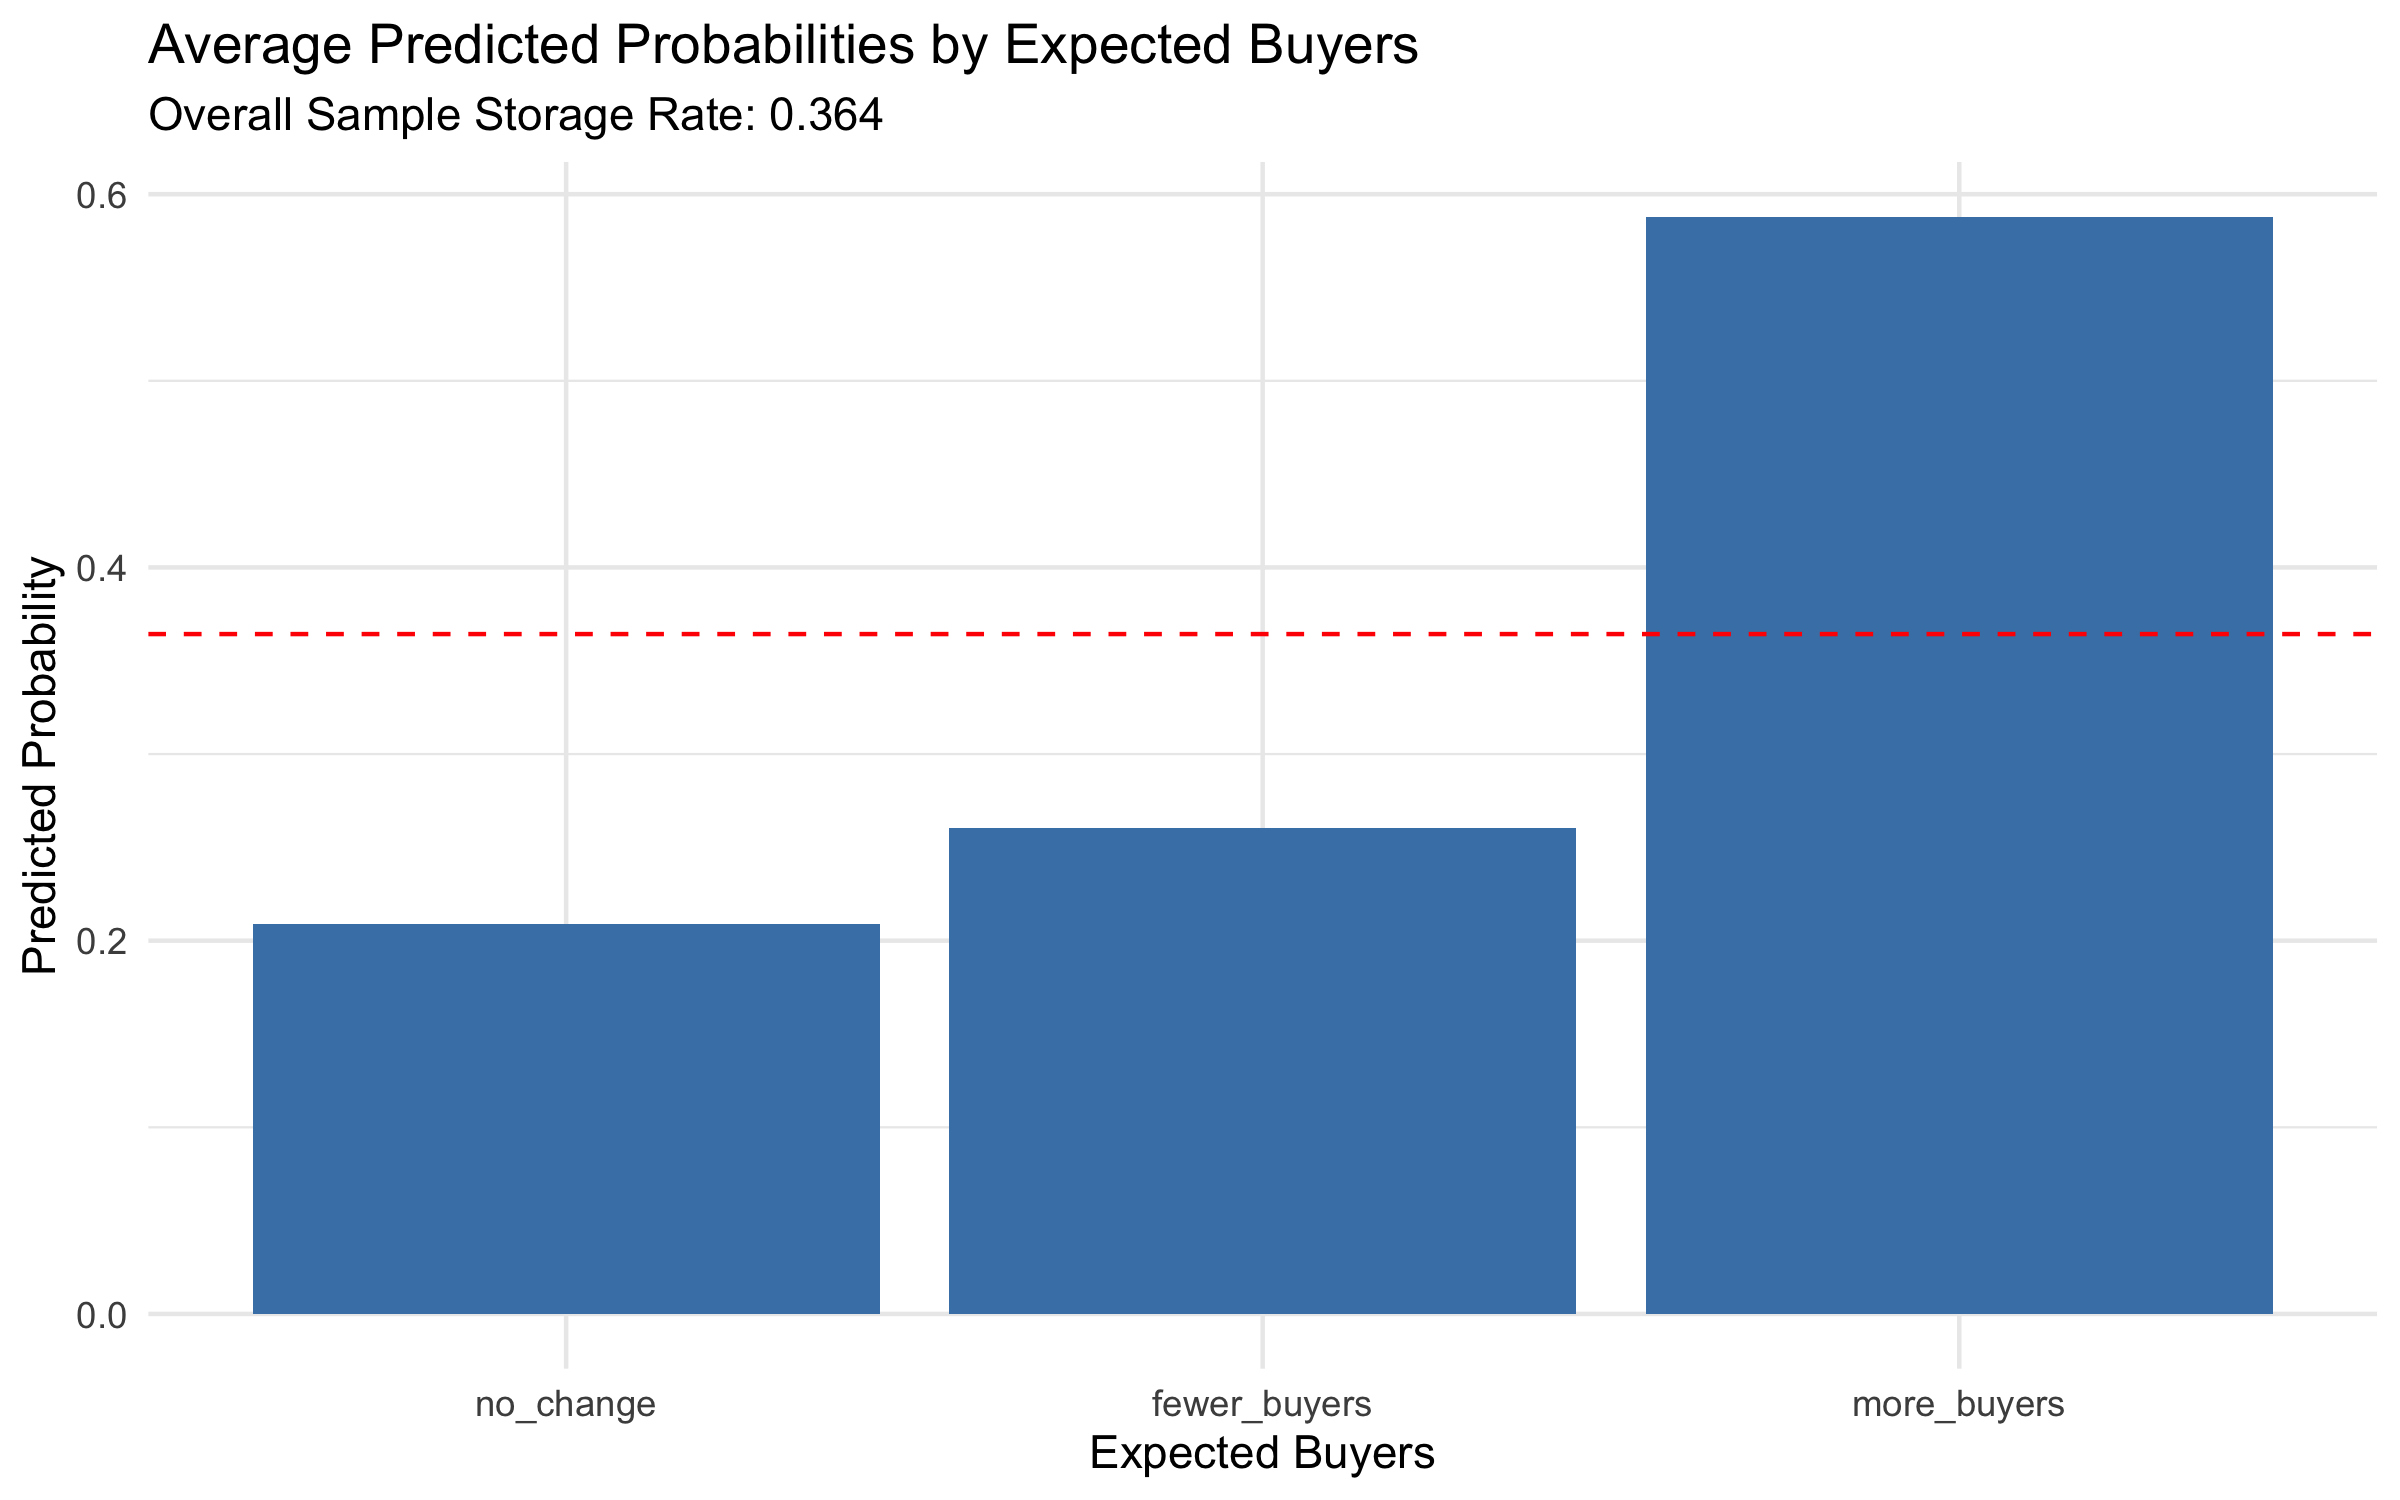
\includegraphics[height=0.28\textheight]{figures/overall_predicted_probs.png}
        \caption{}
    \end{subfigure}\\[2mm]
    
    \begin{subfigure}{\textwidth}
        \centering
        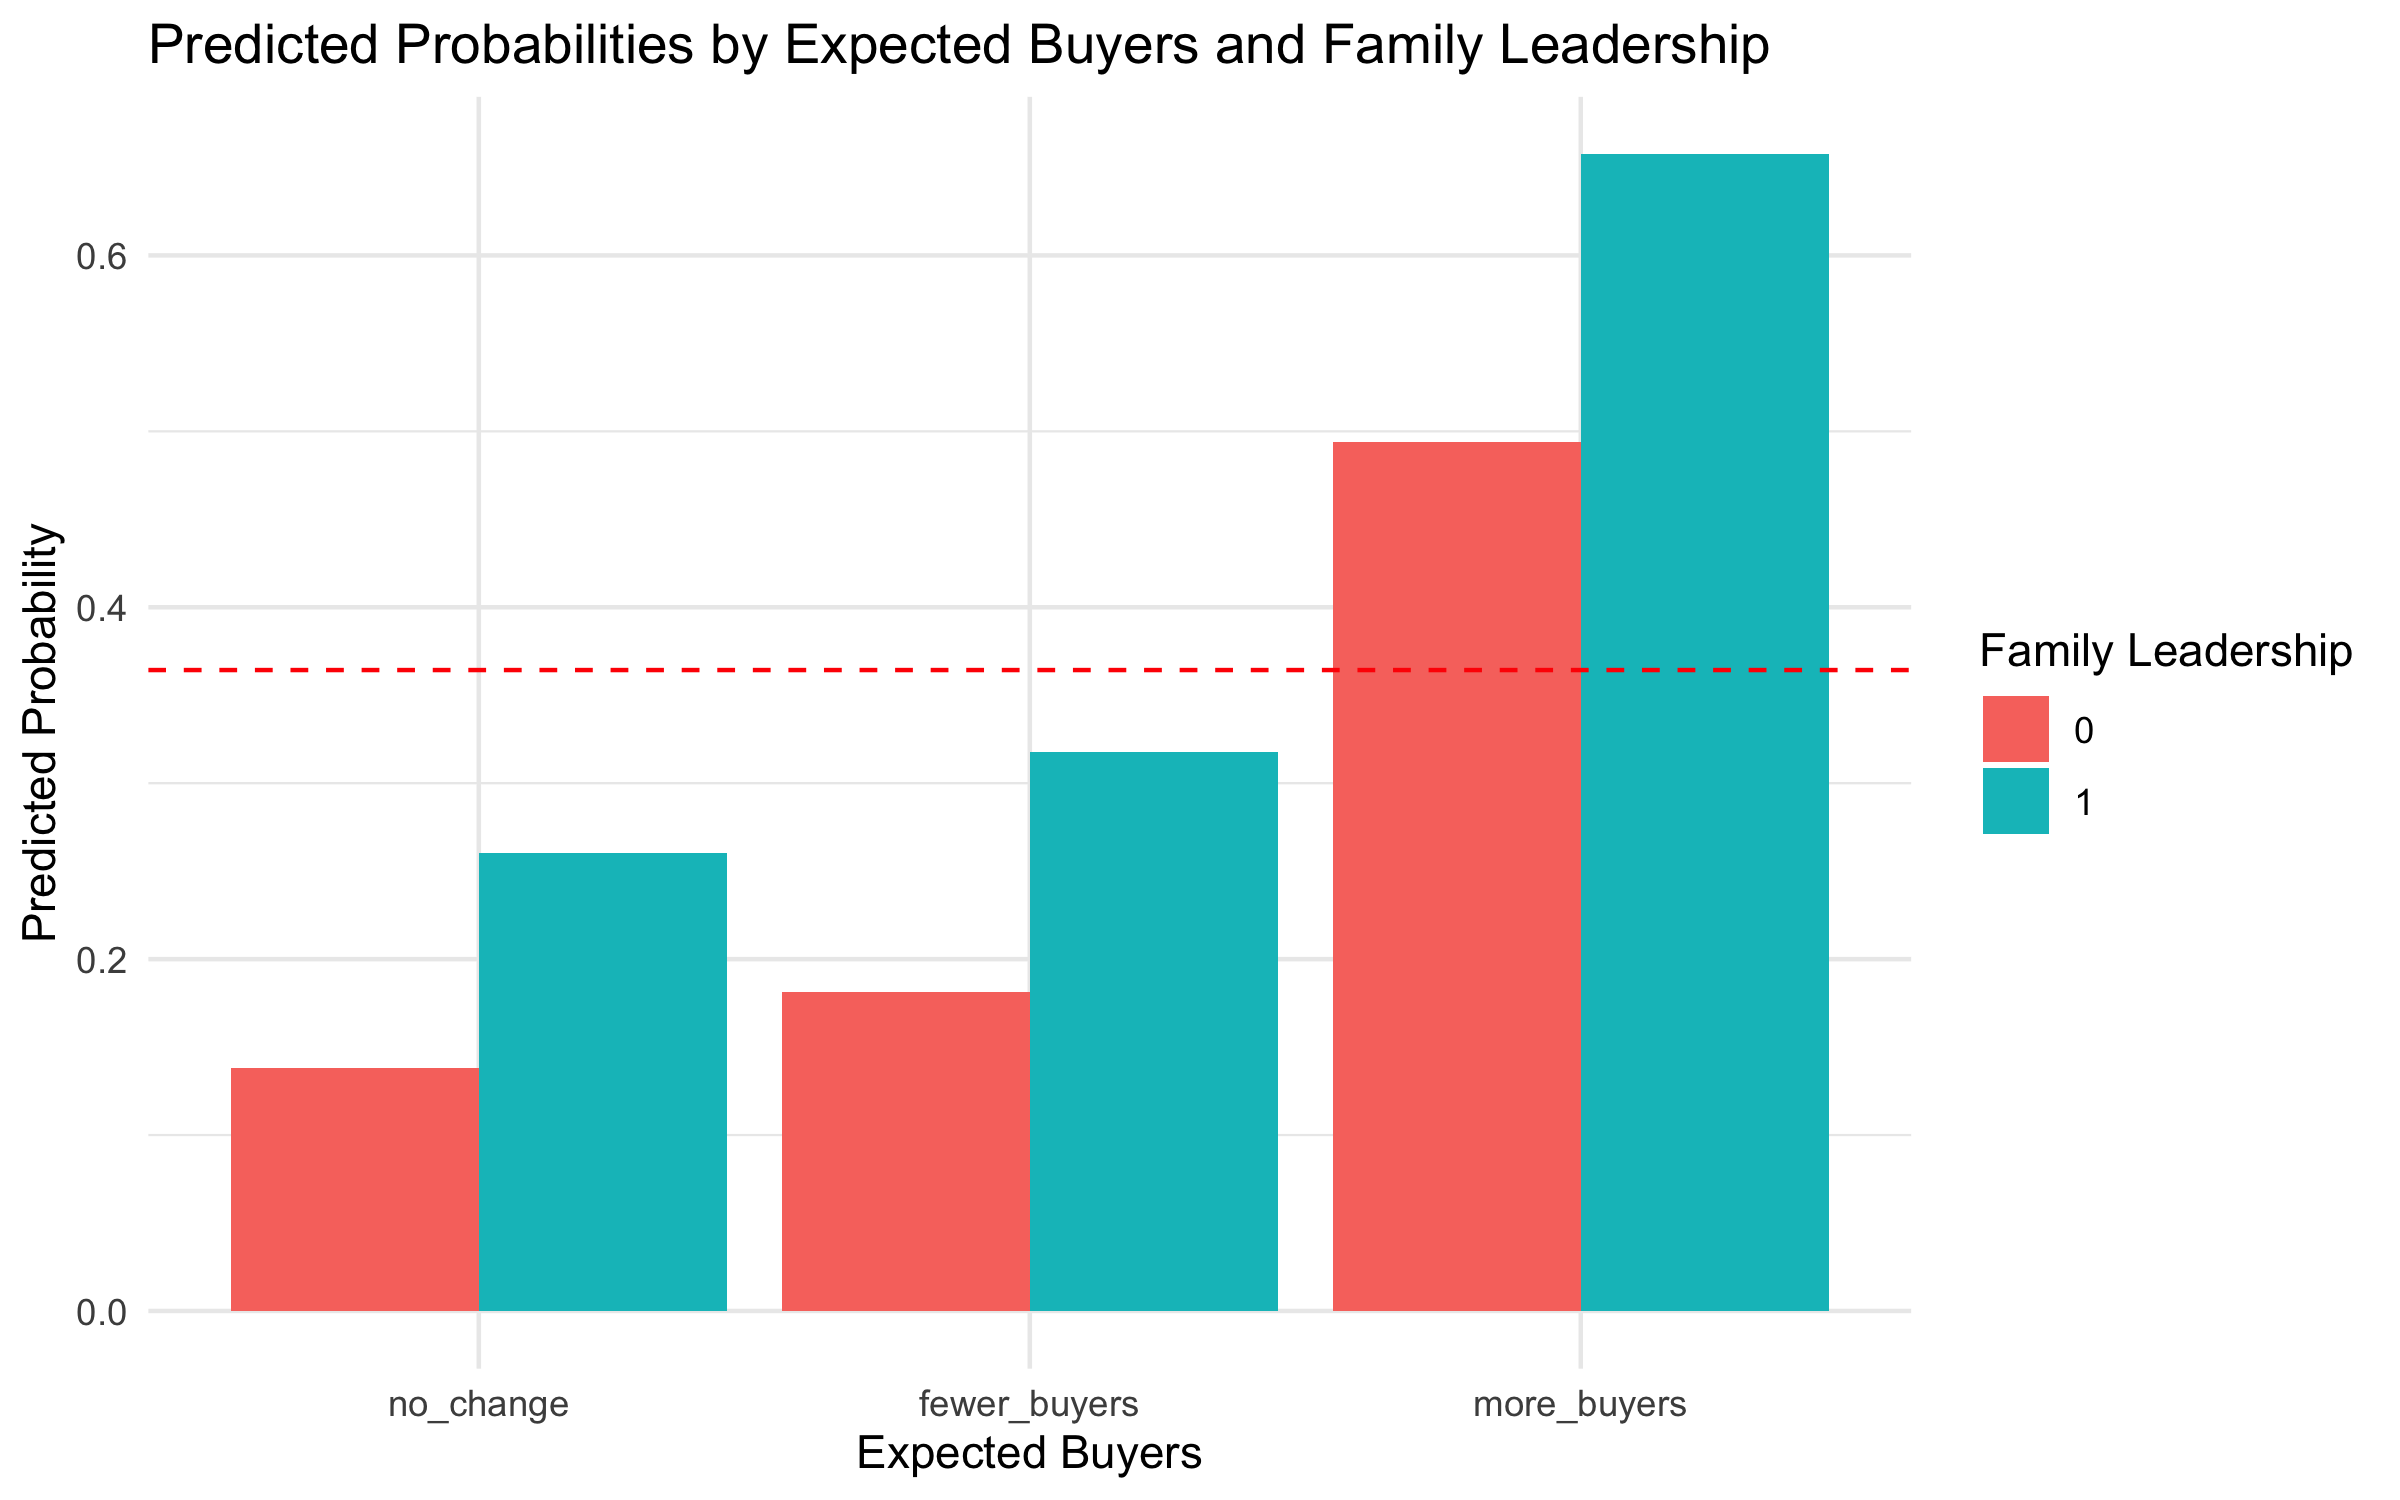
\includegraphics[height=0.28\textheight]{figures/predicted_probs_by_family.png}
        \caption{}
    \end{subfigure}\\[2mm]

    \begin{subfigure}{\textwidth}
        \centering
        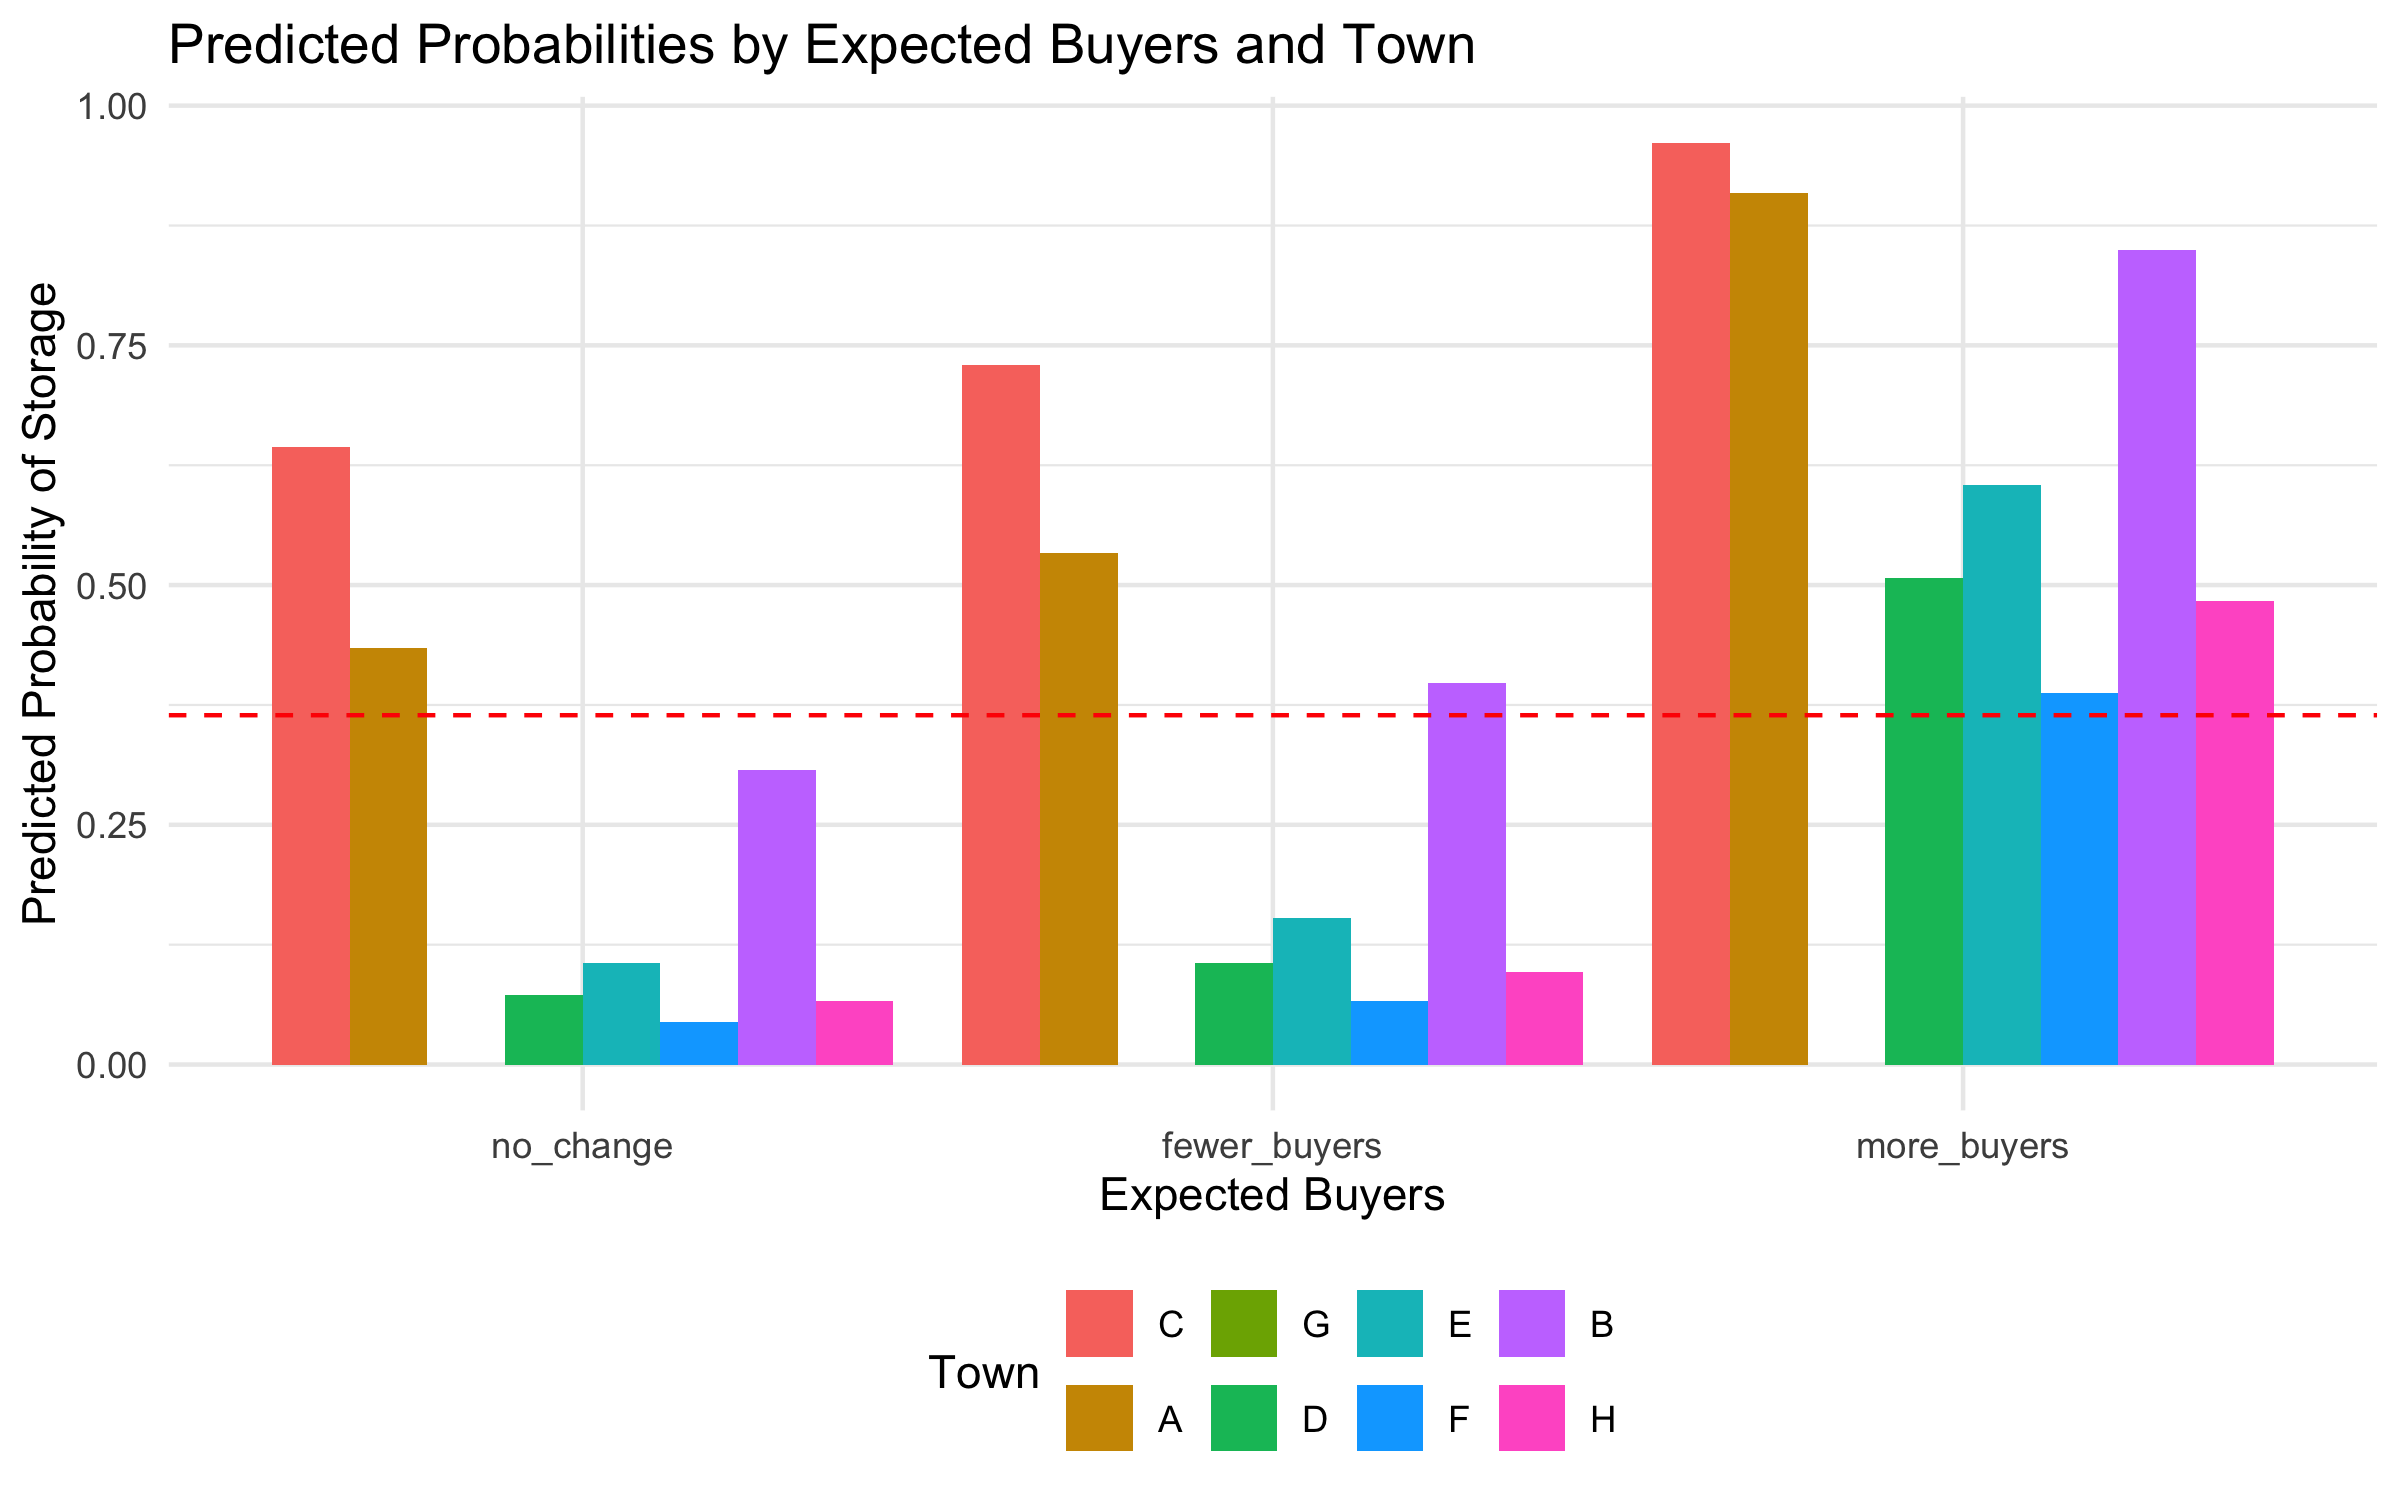
\includegraphics[height=0.28\textheight]{figures/predicted_probs_by_town.png}
        \caption{}
    \end{subfigure}


    \caption{Predicted Probabilities of Storage Usage by Expected Buyer Movement}
    \label{fig:three-images}
\end{figure}





\begin{figure}[ht]
    \centering
    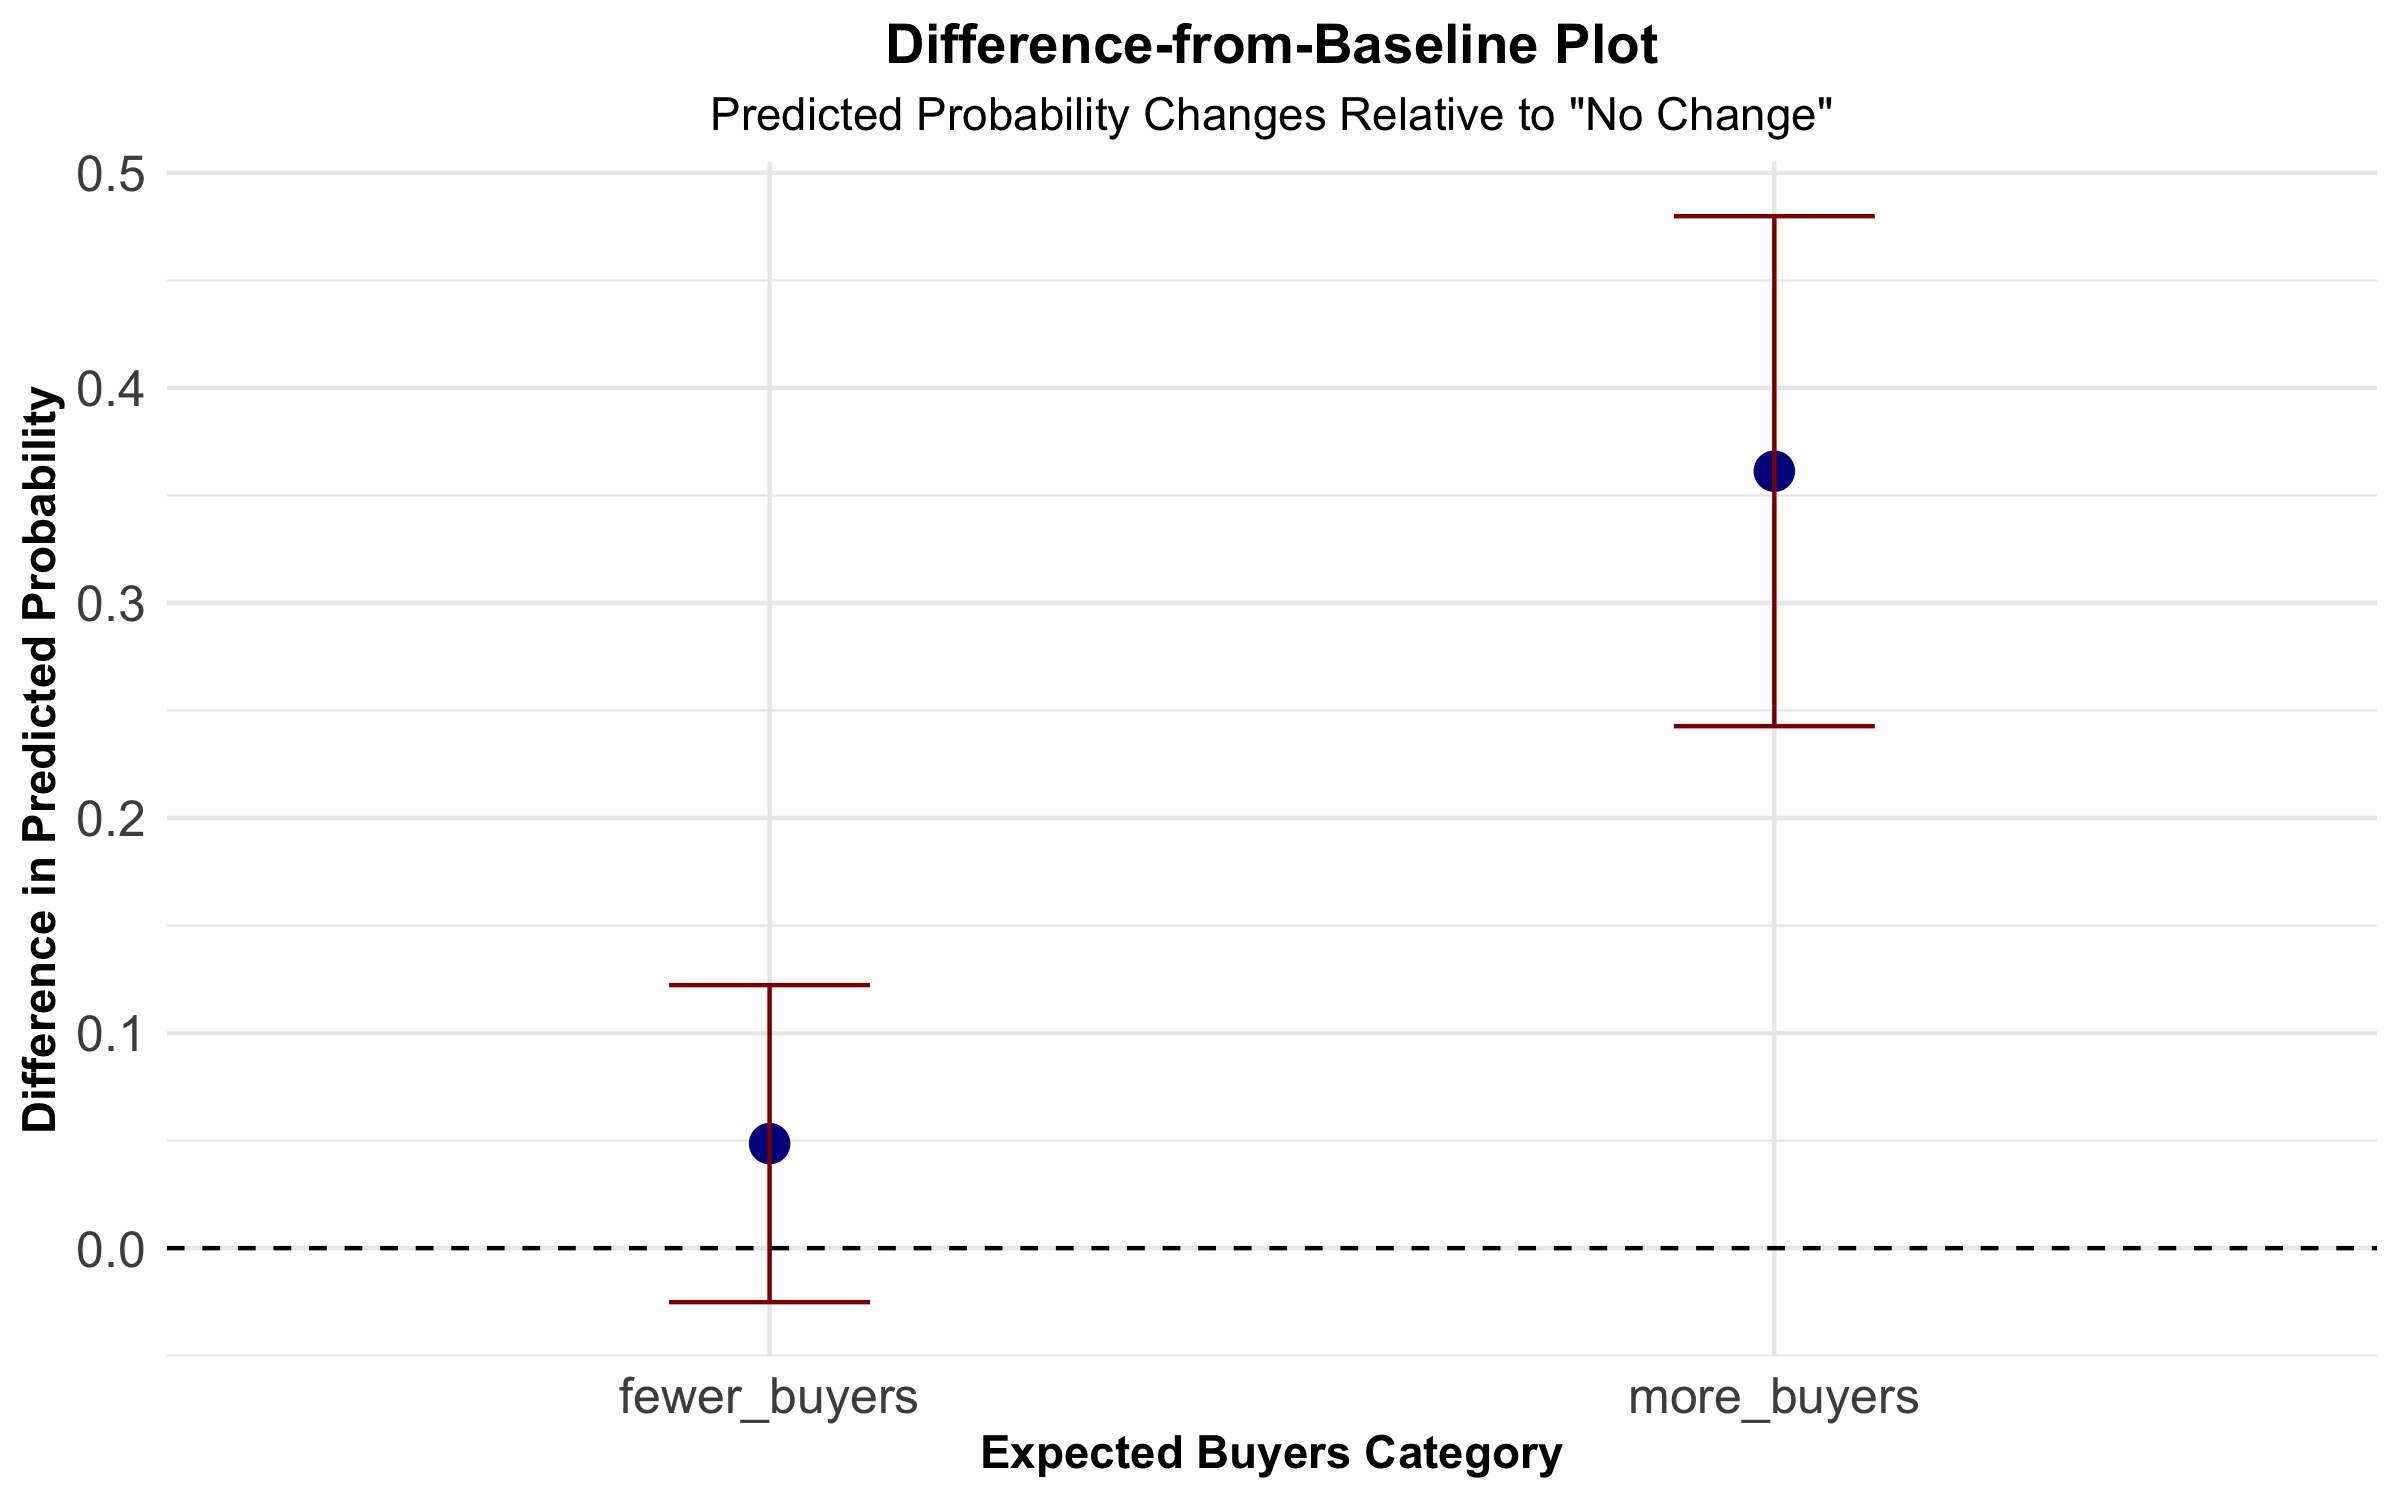
\includegraphics[width=1\textwidth]{figures/filtered_difference_from_baseline_plot.png}
    \caption{Difference-from-Baseline Plot}
    \label{Figure: Difference-from-Baseline Plot}
\end{figure}


\begin{figure}[ht]
\centering
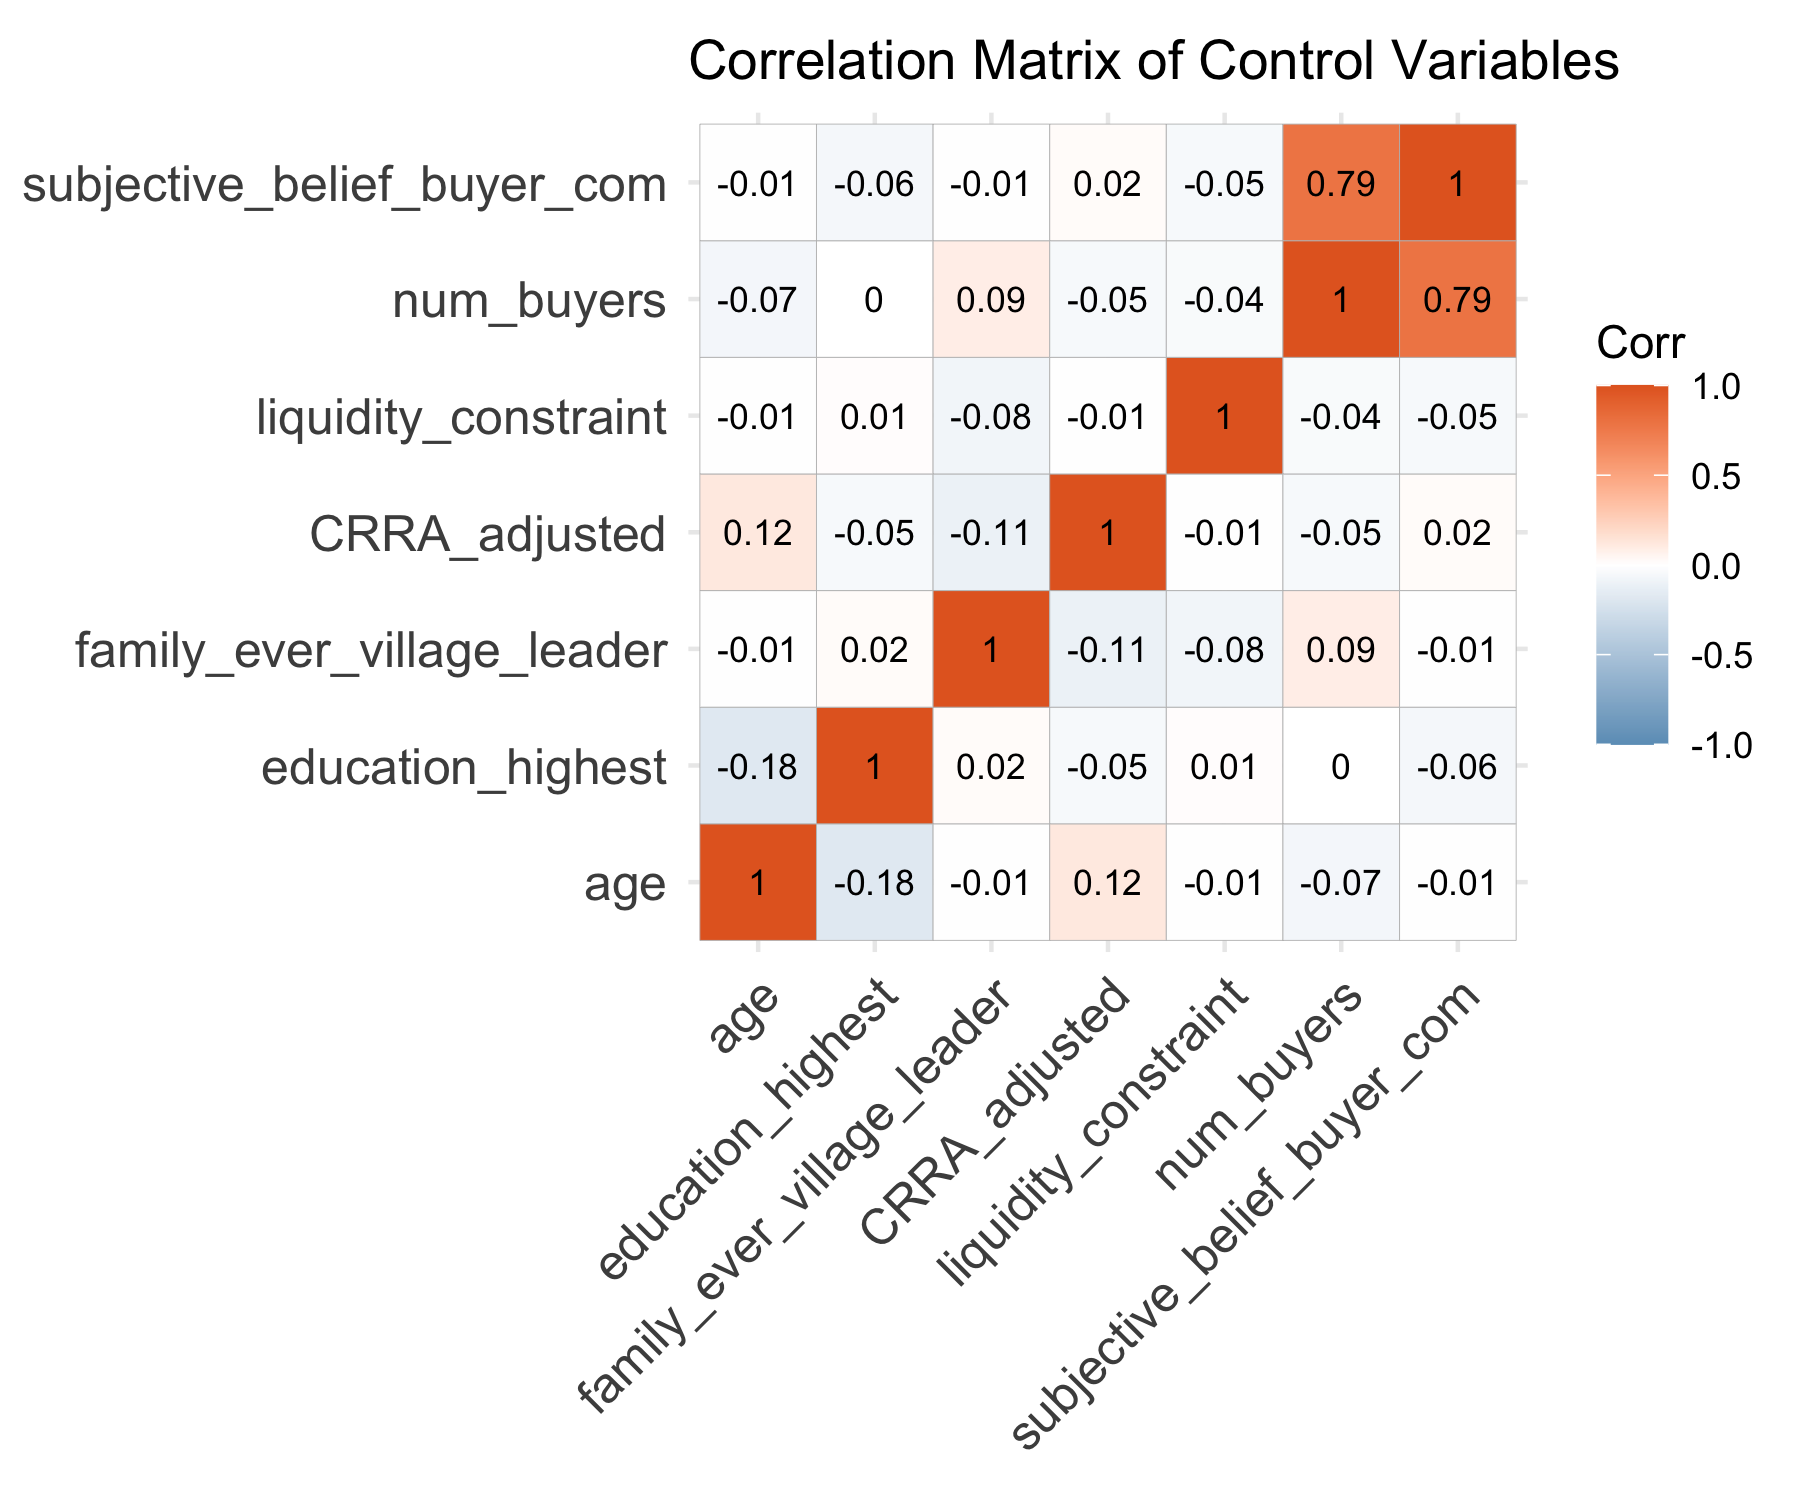
\includegraphics[width=1\textwidth]{figures/correlation_matrix_controls.png}
\caption{Correlation Matrix of Controls}
\label{Figure: Correlation Matrix of Controls}
\end{figure}

Demographic and risk-related factors continue to influence storage decisions in expected directions. Age has a consistently negative impact on storage usage, with AMEs of -0.003 (\(p < 0.1\)), indicating that older individuals are less likely to store their harvest. In contrast, family leadership status remains a strong positive predictor, with an AME of 0.105 (\(p < 0.01\)), suggesting that farmers with family leadership experience are significantly more likely to store their produce. Risk aversion also exerts a significant negative effect on storage decisions, with AMEs of -0.100 (\(p < 0.01\)), reinforcing the tendency of more risk-averse individuals to favor immediate sales over storage due to the uncertainty associated with future prices.

The correlation matrix of control variables, presented in Figure \ref{Figure: Correlation Matrix of Controls}, further contextualizes these findings by illustrating the relationships among key covariates. The negative correlation between age and education level (\(\rho = -0.18\)) is consistent with the observed effect of age on storage behavior, as younger farmers---who tend to have higher education levels---may be more receptive to market-based strategies, such as storage. Similarly, the relatively low correlation between risk aversion (CRRA adjusted) and other covariates suggests that its influence on storage decisions operates independently of other demographic characteristics. Additionally, farmers' subjective beliefs about buyer competition at harvest exhibit a strong positive correlation with the objective number of buyers at harvest (\(\rho = 0.79\)), reinforcing the idea that perceptions of market competition align closely with objective conditions, though they remain distinct factors. The overall low to moderate correlations among control variables reduce concerns about multicollinearity, supporting the reliability of the logistic regression estimates and their implications for storage behavior.



\subsection{Time to Sell: Expected Buyer Movement}

\subsubsection{Hazard Model with AFT}
\noindent 
To examine how farmers' expectations regarding buyer competition, price expectations, logistical factors, and external conditions influence the timing of their sales, I employ an accelerated failure-time (AFT) specification within a hazard model framework, following \cite{albuquerque2024market}. The AFT model is well-suited for analyzing interval-censored survival data, as it estimates the time until an event occurs---in this case, the sale of apples. This model assumes that covariates accelerate or decelerate the time to an event by a constant factor. A positive coefficient for a covariate indicates that it prolongs the time until the sale (delays selling), while a negative coefficient shortens it.

Given that my survey data only records the month of sale, an interval-censoring approach is used to improve the accuracy of selling duration estimates. The hazard model estimates the probability that a farmer sells apples at a given time, conditional on not having sold them earlier. In the AFT framework, the model is reinterpreted to focus on the speed of selling. The hazard rate for farmer \(f\) selling apples \(c\) at time \(t_{c,f}\) is given by:

\begin{equation}
    h_j(t_{c,f}) = h_0(t_{c,f}) \exp\left(-\mathbf{x}_{c,f} \boldsymbol{\beta}\right),
\end{equation}

where \(h_0(t)\) is the baseline hazard function, assumed to follow a Weibull distribution:

\begin{equation}
    h_0(t) = \alpha t^{\alpha-1}.
\end{equation}

The vector \(\mathbf{x}_{c,f}\) includes explanatory variables that influence the timing of sales. The survivor function \(S_j(t)\), which represents the probability that a farmer has not yet sold their apples by time \(t\), is related to the hazard function through:

\begin{equation}
    h_j(t) = -\frac{d \log S_j(t)}{dt}.
\end{equation}

For interval-censored data, the likelihood function is:

\begin{equation}
    \mathcal{L} = \prod_{j=1}^N \left(S_j(t_{i-1}) h(t_i)\right)^{y_{j,i-1}} S_j(t_{i-1})^{1-y_{j,i}},
\end{equation}

where \(y_{j,i} = 1\) if the sale occurs within the interval \(i\).

To control for unobserved location-specific factors such as weather conditions, road infrastructure, and market accessibility, township fixed effects are included in the empirical specification. This improves the model's ability to capture local heterogeneity, although it may reduce estimation efficiency due to the limited number of observations in some townships.


% Table created by stargazer v.5.2.3 by Marek Hlavac, Social Policy Institute. E-mail: marek.hlavac at gmail.com
% Date and time: Tue, Feb 25, 2025 - 17:56:36
\begin{table}[!htbp] \centering 
  \caption{Extended Weibull Survival Models with Controls} 
  \label{} 
\begin{tabular}{@{\extracolsep{5pt}}lcc} 
\\[-1.8ex]\hline 
\hline \\[-1.8ex] 
 & \multicolumn{2}{c}{\textit{Dependent variable:}} \\ 
\cline{2-3} 
\\[-1.8ex] & \multicolumn{2}{c}{Full Sample} \\ 
\\[-1.8ex] & (1) & (2)\\ 
\hline \\[-1.8ex] 
 More Buyers Future & 0.50$^{***}$ & 0.12 \\ 
  & (0.07) & (0.09) \\ 
  & & \\ 
 Less Buyers Future & $-$0.05 & $-$0.21$^{*}$ \\ 
  & (0.07) & (0.11) \\ 
  & & \\ 
 Family Village Leader & 0.05 & $-$0.06 \\ 
  & (0.08) & (0.10) \\ 
  & & \\ 
 Far to Small Storage & $-$0.30$^{***}$ & $-$0.14 \\ 
  & (0.07) & (0.10) \\ 
  & & \\ 
 Far to Large Storage & 0.01 & $-$0.13 \\ 
  & (0.10) & (0.15) \\ 
  & & \\ 
 Storage Purpose: Marketing & 0.33$^{***}$ & $-$0.11 \\ 
  & (0.06) & (0.14) \\ 
  & & \\ 
 Storage Purpose: Bargaining & 0.27$^{***}$ & $-$0.05 \\ 
  & (0.06) & (0.11) \\ 
  & & \\ 
 Education Level & 0.10$^{**}$ & 0.06 \\ 
  & (0.04) & (0.07) \\ 
  & & \\ 
 Number of Buyers & 0.03$^{**}$ & 0.04$^{*}$ \\ 
  & (0.01) & (0.02) \\ 
  & & \\ 
 Constant & 1.08$^{***}$ & 2.31$^{***}$ \\ 
  & (0.14) & (0.24) \\ 
  & & \\ 
\hline \\[-1.8ex] 
Town Fixed Effects & Yes & Yes \\ 
Observations & 549 & 200 \\ 
Log Likelihood & $-$527.73 & $-$283.46 \\ 
$\chi^{2}$ & 493.03$^{***}$ (df = 16) & 50.78$^{***}$ (df = 15) \\ 
\hline 
\hline \\[-1.8ex] 
\textit{Note:}  & \multicolumn{2}{r}{$^{*}$p$<$0.1; $^{**}$p$<$0.05; $^{***}$p$<$0.01} \\ 
\end{tabular} 
\end{table} 


\subsubsection{Results}
\noindent 
Table \ref{tab: extended Survival AFT with controls} presents the results from the AFT Weibull survival model, which estimates the duration (storing time) until farmers sell their apples. Column (1) includes the full sample, while Column (2) focuses exclusively on farmers who utilize storage.

\begin{enumerate}
    \item \textbf{Expected Buyer Competitiveness and Time to Sell:} Farmers' expectations about future buyer competition exhibit distinct effects on their marketing timing. In the full sample (Column 1), anticipating more buyers in the future significantly prolongs the time to sell (\(\beta = 0.50, p<0.01\)), suggesting that farmers expecting increased competition among buyers delay sales, likely in anticipation of higher farm-gate prices. This aligns with the theoretical expectation that greater buyer competition enhances farmers' bargaining power, incentivizing them to wait for more favorable market conditions.
    
    However, among storage users (Column 2), the coefficient on expecting more buyers is smaller and statistically insignificant (\(\beta = 0.12, p>0.1\)), indicating that for farmers already engaged in storage, expectations of further increased competition do not further delay their sales. This suggests that these farmers are already positioned to take advantage of higher prices and are less responsive to incremental changes in buyer expectations.

    Therefore, an optimistic projection on future market competitive conditions mainly encourages storage, but does not necessarily lead to a longer storage time (marketing wait).
    
    Conversely, expectations of fewer buyers in the future exhibit a negative but statistically insignificant coefficient in the full sample (\(\beta = -0.05, p>0.1\)), implying that pessimism about buyer competition does not significantly accelerate selling decisions across all farmers. Among storage users, however, expecting fewer buyers significantly shortens the time to sell (\(\beta = -0.21, p<0.1\)), suggesting that those who store their harvest are more sensitive to potential market downturns and may liquidate their stocks sooner when facing expectations of reduced competition.
    
    \item \textbf{Storage Conditions and Purpose:} 
    Logistical constraints related to storage access significantly influence the decision to store but have limited impact on the duration of storage. Specifically, greater distance to a storage facility reduces the likelihood of storage adoption but does not significantly affect the time apples are kept in storage, which is consistent with theoretical expectations. Farmers located farther from small storage facilities sell significantly earlier than those with closer access (\(\beta = -0.30, p<0.01\)), underscoring that distance imposes a meaningful transaction cost that limits farmers' ability to delay sales for better prices. In contrast, distance to large storage facilities does not have a statistically significant effect, suggesting that large storage infrastructures may be either less frequently utilized or more accessible under different institutional or market arrangements.
    
    The stated purpose of storage also plays a crucial role in determining the time to sell. Farmers who store with the explicit goal of marketing optimization exhibit significantly prolonged selling durations (\(\beta = 0.33, p<0.01\)), supporting the notion that these farmers strategically time their sales to capture better market conditions. Similarly, those who store for bargaining leverage also delay sales (\(\beta = 0.27, p<0.01\)), reinforcing the idea that farmers with stronger price negotiation motives tend to wait longer before selling. However, among storage users (Column 2), neither of these motivations significantly influences time to sell, likely because all individuals in this subsample are already engaged in storage, making other factors more decisive.
    
    \item \textbf{Human Capital and Market Conditions:} Farmers' education levels exhibit a significant and positive relationship with selling time in the full sample (\(\beta = 0.10, p<0.05\)), indicating that more educated farmers are more likely to delay sales, potentially due to better access to market information or stronger financial literacy. However, this effect diminishes among storage users (\(\beta = 0.06, p>0.1\)), suggesting that education primarily affects the initial decision to store rather than the subsequent timing of sales.
    
    The number of buyers at harvest in the market positively affects time to sell in both specifications, though the magnitude is relatively small. In the full sample, each additional buyer visiting during the harvest is associated with a slight delay in selling (\(\beta = 0.03, p<0.05\)), while among storage users, the effect is somewhat stronger (\(\beta = 0.04, p<0.1\)). This implies that market depth during harvest plays a role in prolonging sales, potentially by increasing farmers' confidence in their ability to obtain better prices.
\end{enumerate}

\subsubsection{Summary of Findings}
\noindent 
Overall, the results emphasize the critical role of farmers' expectations about future buyer competition in shaping marketing decisions. While higher expected buyer competition substantially delays sales, this effect is weaker among those who already engage in storage. Logistical constraints, particularly distance to storage, significantly accelerate sales in terms of the decision to store or not, highlighting the role of infrastructure in shaping market participation. Furthermore, farmers' stated storage motivations align with observed selling behavior, as those who store for marketing or bargaining purposes delay sales. Finally, human capital and local market depth exert additional influence, reinforcing the importance of education and buyer availability in determining optimal selling strategies.



\section{Conclusion}
\noindent This empirical analysis sheds light on the critical role of perceived and expected buyer competitiveness in shaping the storage and marketing decisions of smallholder farmers, using data from Fuji apple growers in Yanchang County, Central China. The key findings indicate that farmers' storage decisions are primarily driven by their subjective perceptions of buyer competition, rather than the actual number of buyers at harvest. This result is especially important in light of the existence of buyer collusion behavior that may undermine the apparent benefits of increased buyer presence. Farmers who perceive greater buyer competition at harvest are less likely to engage in storage, as they expect higher prices due to competitive market conditions. This highlights the importance of distinguishing between the observed number of buyers, which often fails to reflect true market competitiveness, and the expected number of buyers, which serves as a practical proxy for perceived competition in the farmers' minds.

In addition to harvest-time perceptions, farmers' expectations regarding future buyer competition significantly influence their storage decisions. Specifically, farmers are more likely to store their produce at harvest when they anticipate increased competition in the future, particularly over the next three months. This suggests that farmers view storage as a strategic tool to capitalize on expected market improvements. While the expectation of stronger competition incentivizes storage, expectations of fewer buyers do not significantly deter storage adoption. This asymmetry suggests that farmers are more responsive to the potential for price increases due to heightened competition than to the risks associated with reduced buyer presence. The findings underscore the role of perceived future market opportunities in shaping storage decisions, emphasizing the dynamic nature of smallholder decision-making in response to both current and anticipated market conditions.

The analysis further highlights the influence of demographic factors, risk preferences, and social capital on storage behavior. Specifically, older farmers and those with higher risk aversion are less likely to adopt storage, which is consistent with the theoretical expectation that more risk-averse individuals prefer immediate sales to mitigate uncertainty. Conversely, family leadership status and education level are positively associated with storage adoption. These factors suggest that farmers with stronger social networks and greater access to market information are more likely to invest in storage, recognizing its value for market timing and price negotiation. This finding indicates that access to storage is not only shaped by financial resources but also by social capital and education, which enhance farmers' ability to navigate market uncertainty and leverage storage as a marketing tool.

In line with these findings, the survival model analysis underscores the critical role of future buyer expectations in shaping marketing behavior. The expectation of increased buyer competition substantially delays sales, as farmers anticipate higher prices. However, this effect is weaker among those who already store their produce, indicating that farmers who are already engaged in storage are less responsive to additional market signals. This suggests that storage adoption provides a strategic buffer against market volatility, enabling farmers to hold out for more favorable prices without the immediate pressure to sell. Additionally, logistical constraints, particularly the distance to storage, significantly accelerate sales, highlighting how infrastructure access shapes market participation and sales timing. Farmers located farther from storage facilities are more likely to sell early, suggesting that the costs associated with storage access influence the timing of their sales. Furthermore, farmers who store for marketing optimization or bargaining leverage are more likely to delay sales, supporting the idea that storage decisions are not solely driven by financial necessity but by strategic considerations to maximize returns.

Lastly, human capital and local market depth exert additional influences on farmers' selling strategies. Education and buyer availability contribute to the farmers' ability to make more informed and market-efficient decisions, which, in turn, affects their storage and selling behaviors. More educated farmers, for instance, are more likely to delay sales, likely due to better access to market information and stronger financial literacy, which enables them to make informed decisions about when and how to sell. This underscores the broader economic forces at play, where access to education and market infrastructure plays a crucial role in shaping farmers' decision-making.

